
%%
%% forked from https://gits-15.sys.kth.se/giampi/kthlatex kthlatex-0.2rc4 on 2020-02-13
%% expanded upon by Gerald Q. Maguire Jr.
%% This template has been adapted by Anders Sjögren to the University
%% Engineering Program in Computer Science at KTH ICT. This adaptation was
%% translation of English headings into Swedish with the addition of Swedish.
%% Many thanks to others who have provided constructive input regarding the template.

% Make it possible to conditionally depend on the TeX engine used
\RequirePackage{ifxetex}
\RequirePackage{ifluatex}
\newif\ifxeorlua
\ifxetex\xeorluatrue\fi
\ifluatex\xeorluatrue\fi

\ifxeorlua
% The following is to ensure that the PDF uses a recent version rather than the typical PDF 1-5
%  This same version of PDF should be set as an option for hyperef

\RequirePackage{expl3}
\RequirePackage{etoolbox}


\ExplSyntaxOn
%pdf_version_gset:n{2.0}
%\pdf_version_gset:n{1.5}

%% Alternatively, if you have a LaTeX newer than June 2022, you can use the following. However, then you have to remove the pdfversion from hyperef. It also breaks hyperxmp. So perhaps it is too early to try using it!
%\DocumentMetadata
%{
%% testphase = phase-I, % tagging without paragraph tagging
% testphase = phase-II % tagging with paragraph tagging and other new stuff.
%pdfversion = 2.0 % pdfversion must be set here.
%}

% Optionally, you can set the uncompress flag to make it easier to examine the PDF
%\pdf_uncompress: % to check the pdf
\ExplSyntaxOff
\else
\RequirePackage{expl3}
\ExplSyntaxOn
%\pdf_version_gset:n{2.0}
\pdf_version_gset:n{1.5}
\ExplSyntaxOff
\fi

%% Define a pair of commands to disable and reenable specific packages - see https://tex.stackexchange.com/questions/39415/unload-a-latex-package
\makeatletter
\newcommand{\disablepackage}[2]{%
  \disable@package@load{#1}{#2}%
}
\newcommand{\reenablepackage}[1]{%
  \reenable@package@load{#1}%
}
\makeatother
%% To avoid the warning: "Package transparent Warning: Loading aborted, because pdfTeX is not running in PDF mode."
\ifxeorlua
\disablepackage{transparent}{}
\fi

%% The template is designed to handle a thesis in English or Swedish
\documentclass[english, bibtex]{kththesis}               % the bibliographic processor to use: biblatex or bibtex
%nomenclature,           % add the option nomenclature
%digitaloutput,          % optimize for digital output (this changes the color palette)
%includeExtraAbstracts, % uncomment to allow abstracts in languages beyond English & Swedish


% if pdflatex \usepackage[utf8]{inputenc}

%% Conventions for todo notes:
% Informational
%% \generalExpl{Comments/directions/... in English}
\newcommand*{\generalExpl}[1]{\todo[inline]{#1}}                

% Language-specific information (currently in English or Swedish)
\newcommand*{\engExpl}[1]{\todo[inline, backgroundcolor=kth-lightgreen40]{#1}} %% \engExpl{English descriptions about formatting}
\newcommand*{\sweExpl}[1]{\todo[inline, backgroundcolor=kth-lightblue40]{#1}}  %% % \sweExpl{Text på svenska}

% warnings
\newcommand*{\warningExpl}[1]{\todo[inline, backgroundcolor=kth-lightred40]{#1}} %% \warningExpl{warnings}

% Hide all template todo notes for the final compile.
\renewcommand\warningExpl[1]{}
\renewcommand\generalExpl[1]{}
\renewcommand\engExpl[1]{}
\renewcommand\sweExpl[1]{}


% \usepackage[style=numeric,sorting=none,backend=biber]{biblatex}
\iftoggle{biblatex}{
    %\usepackage[language=english,bibstyle=authoryear,citestyle=authoryear, maxbibnames=99]{biblatex}
    % Alternatively you might use another style, such as IEEE and use citestyle=numeric-comp  to put multiple citations in a single pair of square brackets
    \usepackage[style=ieee,citestyle=numeric-comp]{biblatex}
    \addbibresource{references.bib}
    %\DeclareLanguageMapping{norsk}{norwegian}
}{
    % The line(s) below are for BibTeX
    \bibliographystyle{bibstyle/myIEEEtran}
    %\bibliographystyle{apalike}
}


% include a variety of packages that are useful
\input{lib/includes}
\input{lib/kthcolors}

%\glsdisablehyper
%\makeglossaries
%\makenoidxglossaries
%%%% Local Variables:
%%% mode: latex
%%% TeX-master: t
%%% End:
% The following command is used with glossaries-extra
\setabbreviationstyle[acronym]{long-short}
% The form of the entries in this file is \newacronym{label}{acronym}{phrase}
%                                      or \newacronym[options]{label}{acronym}{phrase}

\newacronym{auprc}{AUPRC}{area under the precision-recall curve}
\newacronym{auroc}{AUROC}{area under the receiver operating characteristic curve}
\newacronym{cpu}{CPU}{central processing unit}
\newacronym{json}{JSON}{JavaScript Object Notation}
\newacronym{API}{API}{application programming interface}
\newacronym{bert}{BERT}{Bidirectional Encoder Representations from Transformers}
\newacronym{gpu}{GPU}{graphics processing unit}
\newacronym[longplural={large language models}]{llm}{LLM}{large language model}
\newacronym{llmjudge}{LLM-as-a-Judge}{large language model as a judge}
\newacronym{qa}{QA}{question answering}
\newacronym{rag}{RAG}{Retrieval-Augmented Generation}
\newacronym{tfidf}{TF-IDF}{term frequency-inverse document frequency}
\newacronym{UN}{UN}{United Nations}
\newacronym{SDG}{SDG}{Sustainable Development Goal}
                %load the acronyms file

\input{lib/defines}  % load some additional definitions to make writing more consistent

% The following is needed in conjunction with generating the DiVA data with abstracts and keywords using the scontents package and a modified listings environment
%\usepackage{listings}   %  already included

\makeatletter
\let\verbatimsc\@undefined
\let\endverbatimsc\@undefined
\lst@AddToHook{Init}{\hyphenpenalty=50\relax}
\makeatother


\lstnewenvironment{verbatimsc}
    {
    \lstset{%
        basicstyle=\ttfamily\tiny,
        backgroundcolor=\color{white},
        %basicstyle=\tiny,
        %columns=fullflexible,
        columns=[l]fixed,
        language=[LaTeX]TeX,
        %numbers=left,
        %numberstyle=\tiny\color{gray},
        keywordstyle=\color{red},
        breaklines=true,                 % sets automatic line breaking
        breakatwhitespace=true,          % sets if automatic breaks should only happen at whitespace
        %keepspaces=false,
        breakindent=0em,
        %fancyvrb=true,
        frame=none,                     % turn off any box
        postbreak={}                    % turn off any hook arrow for continuation lines
    }
}{}

%% Add some more keywords to bring out the structure more
\lstdefinestyle{[LaTeX]TeX}{
morekeywords={begin, todo, textbf, textit, texttt}
}

%% definition of new command for bytefield package
\newcommand{\colorbitbox}[3]{%
	\rlap{\bitbox{#2}{\color{#1}\rule{\width}{\height}}}%
	\bitbox{#2}{#3}}




% define a left aligned table cell that is ragged right
\newcolumntype{L}[1]{>{\raggedright\let\newline\\\arraybackslash\hspace{0pt}}p{#1}}

% Because backref is not compatible with biblatex
\iftoggle{biblatex}{
    \usepackage[plainpages=false]{hyperref}
}{
    \usepackage[
    backref=page,
    pagebackref=false,
    plainpages=false,
                            % PDF related options
    unicode=true,           % Unicode encoded PDF strings
    bookmarks=true,         % generate bookmarks in PDF files
    bookmarksopen=false,    % Do not automatically open the bookmarks in the PDF reading program
    pdfpagemode=UseNone,    % None, UseOutlines, UseThumbs, or FullScreen
    destlabel,              % better naming of destinations
    pdfencoding=auto,       % for unicode in 
    ]{hyperref}
   %% Removed use of backref package as it is incompatible with using attachfile
}

\usepackage[all]{hypcap}	%% prevents an issue related to hyperref and caption linking

%% Acronyms
% note that nonumberlist - removes the cross references to the pages where the acronym appears
% note that super will set the descriptions text aligned
% note that nomain - does not produce a main glossary, thus only acronyms will be in the glossary
% note that nopostdot - will prevent there being a period at the end of each entry
\usepackage[acronym, style=super, section=section, nonumberlist, nomain,
nopostdot]{glossaries}
\setlength{\glsdescwidth}{0.75\textwidth}
\usepackage[]{glossaries-extra}
\ifinswedish
    %\usepackage{glossaries-swedish}
\fi

%% For use with the README_notes
% Define a new type of glossary so that the acronyms defined in the README_notes document can be distinct from those in the thesis template
% the tlg, tld, and dn will be the file extensions used for this glossary
\newglossary[tlg]{readme}{tld}{tdn}{README acronyms}


\input{lib/includes-after-hyperref}

%\glsdisablehyper
\makeglossaries
%\makenoidxglossaries

% The following bit of ugliness is because of the problems PDFLaTeX has handling a non-breaking hyphen
% unless it is converted to UTF-8 encoding.
% If you do not use such characters in your acronyms, this could be simplified to just include the acronyms file.
\ifxeorlua
%%% Local Variables:
%%% mode: latex
%%% TeX-master: t
%%% End:
% The following command is used with glossaries-extra
\setabbreviationstyle[acronym]{long-short}
% The form of the entries in this file is \newacronym{label}{acronym}{phrase}
%                                      or \newacronym[options]{label}{acronym}{phrase}

\newacronym{auprc}{AUPRC}{area under the precision-recall curve}
\newacronym{auroc}{AUROC}{area under the receiver operating characteristic curve}
\newacronym{cpu}{CPU}{central processing unit}
\newacronym{json}{JSON}{JavaScript Object Notation}
\newacronym{API}{API}{application programming interface}
\newacronym{bert}{BERT}{Bidirectional Encoder Representations from Transformers}
\newacronym{gpu}{GPU}{graphics processing unit}
\newacronym[longplural={large language models}]{llm}{LLM}{large language model}
\newacronym{llmjudge}{LLM-as-a-Judge}{large language model as a judge}
\newacronym{qa}{QA}{question answering}
\newacronym{rag}{RAG}{Retrieval-Augmented Generation}
\newacronym{tfidf}{TF-IDF}{term frequency-inverse document frequency}
\newacronym{UN}{UN}{United Nations}
\newacronym{SDG}{SDG}{Sustainable Development Goal}
                %load the acronyms file
\else
\input{lib/acronyms-for-pdflatex}
\fi

% place holders for languages lacking .lbx files
\input{lib/placeHolder_lbx_files}

% insert the configuration information with author(s), examiner, supervisor(s), ...
\input{custom_configuration}

% read in the plain text definitions, if they exist
\IfFileExists{custom_configuration_plaintext.tex}{\input{custom_configuration_plaintext.tex}}{}


% Enter the English and Swedish keywords here for use in the PDF metadata _and_ for later use
% following the respective abstract.
% Try to put the words in the same order in both languages to facilitate matching. For example:
\EnglishKeywords{Retrieval-Augmented Generation, Hybrid RAG, Query routing, ModernBERT, 2WikiMultihopQA, LLM-as-a-Judge, Cost-performance trade-off}
\SwedishKeywords{Retrieval-Augmented Generation, hybrid-RAG, frågeroutning, ModernBERT, 2WikiMultihopQA, LLM-som-domare, kostnads-prestanda-avvägning}

%%%%% For the oral presentation
%% Add this information once your examiner has scheduled your oral presentation
\presentationDateAndTimeISO{}
\presentationLanguage{}  % generally: eng or swe
\presentationRoom{}
\presentationAddress{}
\presentationCity{Stockholm}

% When there are multiple opponents, separate their names with '\&'
% Opponent's information
%\opponentsNames{A. B. Normal \& A. X. E. Normalè}
\opponentsNames{}

% It is possible to have a cover illustration
%\coverIllustration{figures/image1.png}
% if so, the author might acknowledge this or give the copyright information for it with:
%\coverIllustrationCredit{A. B. Normal}

% Once a thesis is approved by the examiner, add the TRITA number
% The TRITA number for a thesis consists of two parts: a series (unique to each school)
% and the number in the series, which is formatted as the year followed by a colon and
% then a unique series number for the thesis - starting with 1 each year.
%\trita{TRITA -- XXX-EX}{2026:0000}

% Put the title, author, and keyword information into the PDF meta information
\input{lib/pdf_related_includes}


% the custom colors and the commands are defined in defines.tex    
\hypersetup{
	colorlinks  = true,
	breaklinks  = true,
	linkcolor   = \linkscolor,
	urlcolor    = \urlscolor,
	citecolor   = \refscolor,
	anchorcolor = black
}

\ifnomenclature
% The following lines make the page numbers and equations hyperlinks in the Nomenclature list
\renewcommand*{\pagedeclaration}[1]{\unskip, \dotfill\hyperlink{page.#1}{page\nobreakspace#1}}
% The following does not work correctly, as the name of the cross-reference is incorrect
%\renewcommand*{\eqdeclaration}[1]{, see equation\nobreakspace(\hyperlink{equation.#1}{#1})}

% You can also change the page heading for the nomenclature
\renewcommand{\nomname}{List of Symbols Used}

% You can even add customization text before the list
\renewcommand{\nompreamble}{The following symbols will be later used within the body of the thesis.}
\makenomenclature
\fi

%
% The commands below are to configure JSON listings
% 
% format for JSON listings
\colorlet{punct}{red!60!black}
\definecolor{delim}{RGB}{20,105,176}
\definecolor{numb}{RGB}{106, 109, 32}
\definecolor{string}{RGB}{0, 0, 0}

\lstdefinelanguage{json}{
    numbers=none,
    numberstyle=\small,
    frame=none,
    rulecolor=\color{black},
    showspaces=false,
    showtabs=false,
    breaklines=true,
    postbreak=\raisebox{0ex}[0ex][0ex]{\ensuremath{\color{gray}\hookrightarrow\space}},
    breakatwhitespace=true,
    basicstyle=\ttfamily\small,
    extendedchars=false,
    upquote=true,
    morestring=[b]",
    stringstyle=\color{string},
    literate=
     *{0}{{{\color{numb}0}}}{1}
      {1}{{{\color{numb}1}}}{1}
      {2}{{{\color{numb}2}}}{1}
      {3}{{{\color{numb}3}}}{1}
      {4}{{{\color{numb}4}}}{1}
      {5}{{{\color{numb}5}}}{1}
      {6}{{{\color{numb}6}}}{1}
      {7}{{{\color{numb}7}}}{1}
      {8}{{{\color{numb}8}}}{1}
      {9}{{{\color{numb}9}}}{1}
      {:}{{{\color{punct}{:}}}}{1}
      {,}{{{\color{punct}{,}}}}{1}
      {\{}{{{\color{delim}{\{}}}}{1}
      {\}}{{{\color{delim}{\}}}}}{1}
      {[}{{{\color{delim}{[}}}}{1}
      {]}{{{\color{delim}{]}}}}{1}
      {’}{{\char13}}1,
}

\lstdefinelanguage{XML}
{
  basicstyle=\ttfamily\color{blue}\bfseries\small,
  morestring=[b]",
  morestring=[s]{>}{<},
  morecomment=[s]{<?}{?>},
  stringstyle=\color{black},
  identifierstyle=\color{blue},
  keywordstyle=\color{cyan},
  breaklines=true,
  postbreak=\raisebox{0ex}[0ex][0ex]{\ensuremath{\color{gray}\hookrightarrow\space}},
  breakatwhitespace=true,
  morekeywords={xmlns,version,type}% list your attributes here
}

% If you use both listing and lstlisting environments - the following makes them both use the same counter and the same formatting in the List of Listings
\makeatletter
\AtBeginDocument{\let\c@listing\c@lstlisting}
\AtBeginDocument{\let\l@listing\l@lstlisting}
\makeatother

% Change the heading for the "List of Listings" to simply "Listings"
\renewcommand{\lstlistlistingname}{Listings}

% number each listing within the chapter
\numberwithin{listing}{chapter}

\usepackage{subfiles}

% To have Creative Commons (CC) license and logos use the doclicense package
% Note that the lowercase version of the license has to be used in the modifier
% i.e., one of by, by-nc, by-nd, by-nc-nd, by-sa, by-nc-sa, zero.
% For background see:
% https://www.kb.se/samverkan-och-utveckling/oppen-tillgang-och-bibsamkonsortiet/open-access-and-bibsam-consortium/open-access/creative-commons-faq-for-researchers.html
% https://kib.ki.se/en/publish-analyse/publish-your-article-open-access/open-licence-your-publication-cc
\begin{comment}
\usepackage[
    type={CC},
    %modifier={by-nc-nd},
    %version={4.0},
    modifier={by-nc},
    imagemodifier={-eu-88x31},  % to get Euro symbol rather than Dollar sign
    hyphenation={RaggedRight},
    version={4.0},
    %modifier={zero},
    %version={1.0},
]{doclicense}
\end{comment}
\listfiles

\begin{document}
%\selectlanguage{swedish}
%
\selectlanguage{english}

%%% Set the numbering for the title page to a numbering series not in the preface or body
\pagenumbering{alph}
\kthcover
\clearpage\thispagestyle{empty}\mbox{} % empty back of front cover
\titlepage

% If you do not want to have a bookinfo page, comment out the line saying \bookinfopage and add a \cleardoublepage
% If you want a bookinfo page: you will get a copyright notice, unless you have used the doclicense package in which case you will get a Creative Commons license. To include the doclicense package, uncomment the configuration of this package above and configure it with your choice of license.
\bookinfopage

% Frontmatter includes the abstracts and table-of-contents
\frontmatter
\setcounter{page}{1}
\begin{abstract}
% The first abstract should be in the language of the thesis.
% Abstract fungerar på svenska också.
  \markboth{\abstractname}{}
\begin{scontents}[store-env=lang]
eng
\end{scontents}
%%% The contents of the abstract (between the begin and end of scontents) will be saved in LaTeX format
%%% and output on the page(s) at the end of the thesis with information for DiVA facilitating the correct
%%% entry of the meta data for your thesis.
%%% These page(s) will be removed before the thesis is inserted into DiVA.
\engExpl{All theses at KTH are \textbf{required} to have an abstract in both \textit{English} and \textit{Swedish}.}

\engExpl{Exchange students may want to include one or more abstracts in the language(s) used in their home institutions to avoid the need to write another thesis when returning to their home institution.}

\generalExpl{Keep in mind that most of your potential readers are only going to read your \texttt{title} and \texttt{abstract}. This is why the abstract must give them enough information so that they can decide if this document is relevant to them or not. Otherwise, the likely default choice is to ignore the rest of your document.\\
An abstract should stand on its own, \ie no citations, cross-references to the body of the document, acronyms must be spelled out, \ldots .\\Write this early and revise as necessary. This will help keep you focused on what you are trying to do.}

\begin{scontents}[store-env=abstracts,print-env=true]
Retrieval-Augmented Generation (RAG) is the standard approach for grounding large language models in external knowledge, but production systems increasingly combine cheap vector retrieval with more expensive graph-enhanced retrieval. Graph-enhanced retrieval can answer questions whose evidence is split across documents, but is significantly more compute-intensive than vector retrieval. Applying it to every query wastes resources on questions that the cheap path could already handle, while always using vector retrieval misses the questions that genuinely need graph structure.

This thesis studies whether the choice between a cheap vector retrieval mode and a more expensive graph-enhanced retrieval mode can be predicted from the query text alone. The setting is the 2WikiMultihopQA benchmark inside the LightRAG retrieval framework, with LightRAG's Naive mode as the cheap path and its Mix mode as the graph-enhanced path. Routing labels are constructed by executing both retrieval modes on every benchmark question and using a large language model as a judge to compare each mode's answer against the gold answer. The resulting binary routing dataset is split jointly by question type and routing label, and used to train and evaluate two query-only routers: a TF-IDF logistic-regression baseline and a fine-tuned ModernBERT classifier.

On a held-out test split of 193 queries, the ModernBERT router improves on the TF-IDF baseline on every aggregate classification metric, including area under the precision-recall curve (0.769 vs.\ 0.742), balanced accuracy (0.798 vs.\ 0.784), and F1 on the minority class (0.699 vs.\ 0.650), with gains that are stable across three training seeds. Treated as offline routing policies and evaluated along two cost dimensions, both routers route at substantially lower mean cost than always using graph-enhanced retrieval, with the ModernBERT router reducing mean execution time by 39\,\% and mean LLM token usage by 60\,\% relative to the always-graph baseline. The retrieval-mode distinction is therefore partly predictable from the query text alone, and a lightweight encoder classifier is a viable routing layer for adaptive Hybrid RAG.
\end{scontents}

\subsection*{Keywords}
\begin{scontents}[store-env=keywords,print-env=true]
% If you set the EnglishKeywords earlier, you can retrieve them with:
\InsertKeywords{english}
% If you did not set the EnglishKeywords earlier then simply enter the keywords here:
% comma separate keywords, such as: Canvas Learning Management System, Docker containers, Performance tuning
\end{scontents}
\end{abstract}
\cleardoublepage
\babelpolyLangStart{swedish}
\begin{abstract}
    \markboth{\abstractname}{}
\begin{scontents}[store-env=lang]
swe
\end{scontents}
\warningExpl{Inside the following scontents environment, you cannot use a \textbackslash include{filename} as the command rather than the file contents will end up in the for DiVA information. Additionally, you should not use a straight double quote character in the abstracts or keywords, use two single quote characters instead.}
\sweExpl{Alla avhandlingar vid KTH \textbf{måste ha} ett abstrakt på både \textit{engelska} och \textit{svenska}.\\
Om du skriver din avhandling på svenska ska detta göras först (och placera det som det första abstraktet) - och du bör revidera det vid behov.}

\engExpl{If you are writing your thesis in English, you can leave this until the draft version that goes to your opponent for the written opposition. In this way, you can provide the English and Swedish abstract/summary information that can be used in the announcement for your oral presentation.\\If you are writing your thesis in English, then this section can be a summary targeted at a more general reader. However, if you are writing your thesis in Swedish, then the reverse is true – your abstract should be for your target audience, while an English summary can be written targeted at a more general audience.\\This means that the English abstract and Swedish sammnfattning  
or Swedish abstract and English summary need not be literal translations of each other.}

\warningExpl{Do not use the \textbackslash glspl\{\} command in an abstract that is not in English, as my programs do not know how to generate plurals in other languages. Instead, you will need to spell these terms out or give the proper plural form. In fact, it is a good idea not to use the glossary commands at all in an abstract/summary in a language other than the language used in the \texttt{acronyms.tex file} - since the glossary package does \textbf{not} support use of more than one language.}

\engExpl{The abstract in the language used for the thesis should be the first abstract, while the Summary/Sammanfattning in the other language can follow}
\begin{scontents}[store-env=abstracts,print-env=true]
Retrieval-Augmented Generation (RAG) är den vanligaste arkitekturen för att förankra stora språkmodeller i externt material, men i moderna system kombineras ofta billig vektorbaserad sökning med dyrare grafbaserad hämtning. Grafbaserad hämtning kan svara på frågor vars belägg är fördelade över flera dokument, men är väsentligt mer beräkningskrävande än vektorbaserad sökning. Att tillämpa den på varje fråga slösar resurser på frågor som den billigare metoden redan klarar, medan att alltid använda enbart vektorsökning missar de frågor som faktiskt behöver grafstrukturen.

Denna avhandling undersöker om valet mellan ett billigt vektorbaserat hämtningsläge och ett dyrare grafbaserat hämtningsläge kan förutsägas enbart utifrån frågetexten. Experimenten utförs på riktmärket 2WikiMultihopQA i hämtningsramverket LightRAG, där LightRAG:s \emph{Naive}-läge utgör den billiga vägen och dess \emph{Mix}-läge den grafbaserade vägen. Routingetiketter konstrueras genom att köra båda hämtningslägena på varje fråga och låta en stor språkmodell som domare jämföra respektive svar mot facit. Det resulterande binära routingdatasetet delas upp gemensamt efter frågetyp och routingetikett och används för att träna och utvärdera två routrar som endast ser frågetexten: en TF-IDF-baserad logistisk regressionsmodell som baslinje och en finjusterad ModernBERT-klassificerare.

På en testmängd om 193 frågor förbättrar ModernBERT-routern TF-IDF-baslinjen på samtliga aggregerade klassificeringsmått, däribland arean under precision-recall-kurvan (0,769 mot 0,742), balanserad noggrannhet (0,798 mot 0,784) och F1 på minoritetsklassen (0,699 mot 0,650), med skillnader som är stabila över tre träningsfrön. Som offline-routingpolicyer utvärderade längs två kostnadsdimensioner ger båda routrarna betydligt lägre medelkostnad än att alltid använda grafbaserad hämtning, där ModernBERT-routern minskar medelexekveringstiden med 39\,\% och LLM-tokenanvändningen med 60\,\% relativt det dyraste alternativet. Valet av hämtningsläge är därmed delvis förutsägbart enbart utifrån frågetexten, och en lättviktig encoder-klassificerare är ett gångbart routinglager för adaptiv hybrid-RAG.
\end{scontents}
\subsection*{Nyckelord}
\begin{scontents}[store-env=keywords,print-env=true]
% SwedishKeywords were set earlier, hence we can use alternative 2
\InsertKeywords{swedish}
\end{scontents}
\sweExpl{Nyckelord som beskriver innehållet i uppsatsen eller rapporten}
\end{abstract}
\cleardoublepage
\babelpolyLangStop{swedish}
% Note that the \cleardoublepage has to be before the 
% \babelpolyLangStop - otherwise the running headers will not be in the correct language


\engExpl{If you add the class option \texttt{includeExtraAbstracts} in your \texttt{docuemntclass}, then you can enable abstracts/summaries in a number of languages. Include those versions of abstracts that you need.}
\generalExpl{If you are an exchange student, use the relevant language or languages for abstracts for your home university, as this will often avoid the need for writing another thesis for your home university.}
\generalExpl{If you are fluent in other languages, feel free to add the abstracts in one or more of them.}

\engExpl{The set of languages that can be easily included are based on those languages that were used in theses at KTH in the period 2018-2019, along with several others that have been used in theses since.}
\warningExpl{Note that you may need to augment the set of languages used in \texttt{polyglossia} or
\texttt{babel} (see the file \texttt{kththesis.cls}). If you add a new language, when specifying the language for the abstract, use the three-letter ISO 639-2 Code – specifically the "B" (bibliographic) variant of these codes (note that this is the same language code used in DiVA).}

\cleardoublepage
\iftoggle{includeExtraAbstracts}{
% To include abstracts in languages other than English and Swedish:
%  1. Ensure 'includeExtraAbstracts' is an active option in \documentclass.
%  2. Uncomment the relevant '\input' line(s) below.
%  3. Edit the content within the corresponding file in the 'Additional_Abstracts/' folder.
% Include only the abstracts that you want and fill them in as appropriate
% The template will automatically include the information that you entered
%
% Languages in frequency order based on DiVA data from 2025-05-28

% --- Include Spanish abstract ---
%\input{Additional_Abstracts/abstract_spanish}

% --- Include French abstract ---
%\input{Additional_Abstracts/abstract_french}

% --- Include German abstract ---
%\input{Additional_Abstracts/abstract_german}

% --- Include Italian abstract ---
%\input{Additional_Abstracts/abstract_italian}

% --- Include Chinese abstract ---
%\input{Additional_Abstracts/abstract_chinese}

% --- Include Norwegian abstract ---
%\input{Additional_Abstracts/abstract_norweign}

% --- Include Catalan abstract ---
%\input{Additional_Abstracts/abstract_catalan}

% --- Include Finnish abstract ---
%\input{Additional_Abstracts/abstract_finnish}

% --- Include Portuguese abstract ---
%\input{Additional_Abstracts/abstract_chinese}

% --- Include Dutch abstract ---
%\input{Additional_Abstracts/abstract_dutch}

% --- Include Swahili / Kiswahili summary ---
%\input{Additional_Abstracts/abstract_swahili}

% --- Include Russian summary ---
%\input{Additional_Abstracts/abstract_russian}

% --- Include Polish abstract ---
%\input{Additional_Abstracts/abstract_polishn}

% --- Include Ukrainian abstract ---
%\input{Additional_Abstracts/abstract_ukrainian}

% --- Include Hindi abstract ---
%\input{Additional_Abstracts/abstract_hindi}

% --- Include Danish abstract ---
%\input{Additional_Abstracts/abstract_danish}

% --- Include Estonian abstract ---
%\input{Additional_Abstracts/abstract_estonian}

% --- Include Slovak abstract ---
%\input{Additional_Abstracts/abstract_slovak}

% --- Include Serbian abstract ---
%\input{Additional_Abstracts/abstract_serbian}

% --- Include Bosnian abstract ---
%\input{Additional_Abstracts/abstract_bosnian}

%% missing many languages



}{} %% End the iiftoggle{includeExtraAbstracts}

\section*{Acknowledgments}
\markboth{Acknowledgments}{}
\sweExpl{Författarnas tack}

\engExpl{It is nice to acknowledge the people that have helped you. It is
  also necessary to acknowledge any special permissions that you have gotten –
  for example, getting permission from the copyright owner to reproduce a
  figure. In this case, you should acknowledge them and this permission here
  and in the figure’s caption. \\
  Note: If you do \textbf{not} have the copyright owner’s permission, then you \textbf{cannot} use any copyrighted figures/tables/\ldots . Unless stated otherwise all figures/tables/\ldots are generally copyrighted.
}
\sweExpl{I detta kapitel kan du ev nämna något om
  din bakgrund om det påverkar rapporten på något sätt. Har du t ex inte
  möjlighet att skriva perfekt svenska för att du är nyanländ till landet kan
  det vara på sin plats att nämna detta här. OBS, detta får dock inte vara en
  ursäkt för att lämna in en rapport med undermåligt språk, undermålig grammatik och
  stavning (t ex får fel som en automatisk stavningskontroll och
  grammatikkontroll kan upptäcka inte förekomma)\\
En dualism som måste hanteras i hela rapporten och projektet
}

\engExpl{To ensure academic transparency, you must report whether and how generative AI has been used in your examinable work.  This includes any new content, including, but not limited text, images, tables, or code.}
\sweExpl{För att säkerställa akademisk transparens måste du rapportera om och hur generativ AI har använts i ditt examinerbara arbete. Detta inkluderar allt nytt innehåll, inklusive, men inte begränsat till, text, bilder, tabeller eller kod.}

I would like to thank my KTH supervisor Arvid Eriksson and my Ericsson supervisor Peng Zhang for their guidance, feedback, and continuous support throughout this thesis project.

\acknowlegmentssignature

\fancypagestyle{plain}{}
\renewcommand{\chaptermark}[1]{ \markboth{#1}{}} 
\tableofcontents
  \markboth{\contentsname}{}

\cleardoublepage
\listoffigures

\cleardoublepage

\listoftables
\cleardoublepage
% Align the text expansion of the glossary entries
\newglossarystyle{mylong}{%
  \setglossarystyle{long}%
  \renewenvironment{theglossary}%
     {\begin{longtable}[l]{@{}p{\dimexpr 2cm-\tabcolsep}p{0.8\hsize}}}% <-- change the value here
     {\end{longtable}}%
 }
%\glsaddall
%\printglossaries[type=\acronymtype, title={List of acronyms}]
\printglossary[style=mylong, type=\acronymtype, title={List of acronyms and abbreviations}]

% if the nomenclature option was specified, then include the nomenclature page(s)
\ifnomenclature
    \cleardoublepage
    % Output the nomenclature list
    \printnomenclature
\fi

%% The following label is essential to know the page number of the last page of the preface
%% It is used to compute the data for the "For DIVA" pages
\label{pg:lastPageofPreface}
% Mainmatter is where the actual contents of the thesis goes
\mainmatter
\glsresetall
\renewcommand{\chaptermark}[1]{\markboth{#1}{}}
\selectlanguage{english}
\chapter{Introduction}
\label{ch:introduction}

This chapter introduces the thesis topic and motivates the problem studied in this thesis project. Section~\ref{sec:background} gives the necessary background in retrieval-augmented question answering and the cost of different retrieval modes. Section~\ref{sec:problem} defines the problem and research question. Section~\ref{sec:purpose} states the purpose of the work, Section~\ref{sec:goals} presents the goals, Section~\ref{sec:researchMethodology} outlines the research methodology, Section~\ref{sec:delimitations} defines the delimitations, and Section~\ref{sec:structure} describes the structure of the rest of the thesis.

\section{Background}
\label{sec:background}

\Gls{rag} has become a common architecture for grounding \gls{llm} outputs in external documents, especially when the relevant information is private, domain-specific, or changes after model pretraining \cite{gao2023ragsurvey}. A typical \gls{rag} system retrieves text passages from a corpus and conditions the generator on those passages, making the language model less dependent on memorized knowledge.

The simplest retrieval layer is vector similarity search over document chunks. It is efficient and often effective for local factual questions, but it can struggle when a query depends on linking evidence across documents, resolving relationships between entities, or comparing distributed attributes. Multi-hop question answering benchmarks are designed around exactly this regime, in which the answer can only be derived by chaining several supporting facts together. Graph-enhanced \gls{rag} systems address this by introducing structured representations of entities, relations, or higher-level document organization. Recent systems such as GraphRAG and LightRAG show how graph-based structure can support retrieval beyond vector similarity chunks \cite{edge2024graphrag,lightrag2024}.

Richer retrieval is not free, though. Graph construction, graph traversal, larger context assembly, and additional language-model calls all add to the cost of retrieval. At Ericsson, where internal technical repositories are large and fragmented, graph-enhanced retrieval may improve answer quality for difficult questions, but applying it to every query can waste computational power on questions that cheaper vector retrieval already handles \cite{jeong2024adaptiverag,hu2024routerbench}.

This tension motivates adaptive retrieval. Self-RAG and Adaptive-RAG argue that retrieval behavior should depend on the query rather than follow a fixed policy \cite{asai2023selfrag,jeong2024adaptiverag}. The same cost-performance reasoning appears in \emph{model routing}, where a router decides for each query whether a powerful but computationally expensive language model is needed or whether a cheaper, smaller one would be sufficient \cite{hu2024routerbench}.

The question studied here is narrower than general model routing. Instead of routing between different language models, the project routes between retrieval modes inside a fixed Hybrid \gls{rag} setting. The low-cost path is LightRAG's \emph{Naive} mode, which uses only vector retrieval, and the high-cost path is LightRAG's \emph{Mix} mode, which combines vector retrieval with graph-enhanced retrieval. The routing layer is intentionally lightweight, because if the router itself requires a computationally expensive model, much of the intended efficiency gain is lost.

\section{Research problem}
\label{sec:problem}

The problem approached in this thesis is whether the choice between cheap vector retrieval and graph-enhanced retrieval in Hybrid \gls{rag} can be made before retrieval runs, from the query text alone. In LightRAG, this is operationalized as \emph{Naive} retrieval versus \emph{Mix} retrieval. Prior work motivates both graph-based \gls{rag} and adaptive retrieval \cite{edge2024graphrag,lightrag2024,asai2023selfrag,jeong2024adaptiverag}, but does not quantify how well this choice can be predicted in advance.

\subsection{Problem definition}
\label{sec:problemDefinition}

The research problem is to decide, for a given query, whether cheap vector retrieval suffices or whether graph-enhanced retrieval is required.

The scientific issue is whether retrieval need is predictable from the query alone. If it depends mostly on what the retriever surfaces for each query, a router that sees only the query text cannot anticipate it. If it depends at least partly on how the question is phrased, a supervised classifier may learn a useful decision boundary.

\subsection{Research question}
\label{sec:researchQuestion}

Within a fixed Hybrid \gls{rag} setting, how well can a lightweight query-only classifier predict the required retrieval mode from the query text alone, and how does that predictability translate into the cost--performance trade-off of an adaptive routing policy?

The research question is further split into the following sub-questions:

\begin{itemize}
    \item How well does a fine-tuned encoder-only classifier predict the judged routing label compared to a \gls{tfidf} logistic-regression baseline?
    \item When the classifier scores are turned into a thresholded routing policy, how does the policy's cost--performance trade-off compare against static baseline policies?
    \item Is the routing signal concentrated in particular question types, or does it generalize across them?
\end{itemize}

\section{Purpose}
\label{sec:purpose}
The purpose is to investigate whether retrieval-mode selection in a Hybrid \gls{rag} system can be made adaptive without moving the routing decision into another expensive model call. Graph-enhanced retrieval should be used when it is needed, but avoided when vector retrieval already suffices.

The question is whether the need for graph-enhanced retrieval is predictable enough from the query text that a lightweight classifier can confidently route each query to the sufficient mode. The contribution is therefore empirical, asking whether the vector-sufficient versus graph-required distinction can be learned in a fixed experimental setting.



\section{Goals}
\label{sec:goals}
The main goal is to design and evaluate a learned routing layer that predicts whether a query should use LightRAG's \emph{Naive} or \emph{Mix} retrieval mode. Four concrete objectives structure the work.

\begin{enumerate}
\item Implement a reproducible pipeline for preparing samples from a multi-hop QA benchmark, indexing them in LightRAG, and executing both \emph{Naive} and \emph{Mix} retrieval modes.
\item Construct a supervised routing dataset by labeling each query according to the minimum viable retrieval mode, using \gls{llmjudge} to compare retrieval outputs against benchmark answers.
\item Train lightweight query-only routers, including a ModernBERT-based classifier and a classical \gls{tfidf} logistic-regression baseline, to predict whether graph-enhanced retrieval is required.
\item Evaluate the routers both as held-out classifiers, using metrics such as \gls{auprc} and F1 on the minority class with a majority-class baseline, and as thresholded routing policies measured against always-\emph{Naive} and always-\emph{Mix} baselines on cost metrics including mean routed execution time and mean routed LLM token usage.
\end{enumerate}

\section{Research methodology}
\label{sec:researchMethodology}

This thesis is a quantitative empirical study on a public multi-hop question-answering benchmark, as is common for evaluating retrieval and routing methods. The predictability of retrieval-mode selection from the query text will be evaluated by training query-only routers on judged routing labels and obtaining classification metrics on held-out data, such as \gls{auprc}, balanced accuracy, and F1 on the minority class. The same routers will additionally be evaluated as thresholded routing policies and compared against static baseline policies along cost metrics. Bootstrap confidence intervals will be used to estimate the uncertainty of these metrics. Comparisons between the learned routers and the static baselines will then be used to answer the research question.

\section{Delimitations}
\label{sec:delimitations}

The scope is deliberately limited to query-only retrieval-mode routing. The router receives the query text as input and does not inspect retrieved documents, intermediate graph state, answer drafts, or model uncertainty after generation. This makes the routing problem cheaper and cleaner, but it means the project does not evaluate routers that adapt after retrieval has already begun.

The retrieval setting is LightRAG with two modes: \emph{Naive} and \emph{Mix}. These operationalize the broader vector-versus-graph distinction, but results should not be assumed to transfer automatically to every Hybrid \gls{rag} framework.

The primary benchmark is 2WikiMultihopQA \cite{ho2020twowiki}, chosen because it is public, provides supporting evidence, and makes the experiment reproducible without depending on confidential data. Ericsson documentation motivates the industrial problem but is not the core benchmark.

Routing labels come from \gls{llmjudge} and are treated as judged supervision, not absolute ground truth. Cases where neither retrieval mode produces a correct answer are excluded from router training.

\section{Structure of the thesis}
\label{sec:structure}

Chapter~\ref{ch:background} presents the technical and scientific background on \gls{rag}, graph-enhanced retrieval, adaptive retrieval, query routing, ModernBERT, and related work. Chapter~\ref{ch:methods} describes the experimental method, including data preparation, LightRAG execution, label generation, model training, and evaluation design. Chapter~\ref{ch:implementation} describes the implementation, presents the held-out classification and cost--performance experiments, reports the results, and discusses what they imply about the predictability of retrieval-mode selection. Chapter~\ref{ch:conclusionsAndFutureWork} concludes with answers to the research question and suggestions for future work.

\cleardoublepage
\chapter{Background}
\label{ch:background}

This chapter introduces the technical and scientific concepts that the rest of the thesis builds on. Section~\ref{sec:backgroundRag} describes \gls{rag}, why it is needed for grounding large language model outputs, and how the components fit together. Section~\ref{sec:backgroundHybridGraph} contrasts vector retrieval with graph-enhanced retrieval, including the two LightRAG retrieval modes used in this thesis. Section~\ref{sec:backgroundAdaptiveRetrieval} describes adaptive retrieval and query routing. Section~\ref{sec:backgroundEncoderClassifiers} introduces the language models and text classifiers used by the router. Section~\ref{sec:relatedWork} positions the thesis in relation to prior work.

\section{Retrieval-augmented generation}
\label{sec:backgroundRag}

Large language models encode an enormous amount of general knowledge in their parameters, but they have two limitations relevant to industrial question answering. They cannot access information that was not part of their training data, which makes them unable to answer questions over private or company-internal documents, and they have a tendency to hallucinate, generating fluent but factually incorrect answers when asked about content outside their training distribution \cite{gao2023ragsurvey}. \Gls{rag} addresses both problems by retrieving relevant passages from an external corpus at query time and conditioning the language model on those passages, which both gives the model access to information beyond its training data and lets it ground its answers in cite-able sources \cite{lewis2020rag,gao2023ragsurvey}.

The original \gls{rag} formulation by Lewis et al.\ \cite{lewis2020rag} treats retrieval and generation jointly as a latent-variable problem. Given a query \(q\), a retriever returns a set of documents \(\mathcal{D}_k(q)\), and the generator produces an answer \(a\) by marginalizing over which document was retrieved, as in
\begin{equation}
\label{eq:ragGeneration}
p(a \mid q) =
\sum_{d \in \mathcal{D}_k(q)}
p_\theta(a \mid q,d)\,p_\eta(d \mid q).
\end{equation}
Here \(p_\eta(d \mid q)\) is the retriever, parameterized by \(\eta\), which assigns a probability to each candidate document given the query, and \(p_\theta(a \mid q, d)\) is the generator, parameterized by \(\theta\), which produces the answer given the query and a retrieved document. Equation~\ref{eq:ragGeneration} is not how every modern \gls{rag} system is implemented in practice, but it makes one point that matters for this thesis explicit. Which documents the retrieval system surfaces directly determines what the generator can answer.

For industrial question answering the motivation is concrete. At Ericsson, internal technical documents cannot be assumed to appear in any public language-model pretraining corpus, so a \gls{rag} system is needed to ground answers in company-controlled knowledge. The same is true of many other domain-specific settings, which is why \gls{rag} has become a standard architecture for grounded question answering over private corpora \cite{gao2023ragsurvey}.

Many real questions cannot be answered from a single passage. Multi-hop question answering benchmarks such as HotpotQA, 2WikiMultihopQA, and MuSiQue are constructed around questions whose answers require combining information from multiple supporting documents \cite{yang2018hotpotqa,ho2020twowiki,trivedi2022musique}. For example, a question of the form \emph{``Who is the spouse of the director of film X?''} requires the system first to identify the director of \(X\), then to look up that person, and finally to retrieve their spouse. A retriever that scores each document independently against the query may surface only part of the chain.

\section{Graph-enhanced retrieval}
\label{sec:backgroundHybridGraph}

Most practical \gls{rag} systems start with vector retrieval. Documents are split into chunks, each chunk is encoded into a dense vector by an embedding model, and at query time the chunks whose vectors are closest in the embedding space to the query's vector are returned to the generator \cite{lewis2020rag,karpukhin2020dpr}. This is fast and works well when the answer is contained inside a single passage that resembles the query.

Vector retrieval is weaker when the required evidence is split across multiple documents or depends on relationships between entities. Closeness in the embedding space measures local textual similarity, not the structure that links documents together. As a result, matching the query against individual chunks can surface passages that are each relevant on their own but together still miss the full answer chain.

\subsection{Graph-based RAG systems}
\label{sec:backgroundGraphSystems}

Graph-based \gls{rag} systems address this limitation by constructing a graph over the corpus before any query is asked. Nodes correspond to entities, chunks, or higher-level summaries, and edges correspond to relations between them. At query time the system can then retrieve evidence by traversing this graph rather than only matching the query against individual chunks.

GraphRAG \cite{edge2024graphrag} extracts entities and their relations from each chunk using a language model, builds a knowledge graph over the entire corpus, and groups closely related entities into communities. Each community is summarized into a higher-level description, which can be used to answer queries that span large parts of the corpus. LightRAG \cite{lightrag2024} follows a similar two-level idea, but is designed to be faster and easier to deploy. It also extracts an entity-relation graph during indexing and uses it together with vector chunks at retrieval time, and it exposes several retrieval modes that vary in how heavily they use this graph. The key practical difference for this thesis is that LightRAG explicitly exposes a cheap vector-only retrieval mode and a more expensive graph-enhanced mode in the same framework, which makes it possible to compare the two modes on identical inputs.

Graph-enhanced retrieval is significantly more computationally expensive than pure vector retrieval. Building the graph requires many language-model calls during indexing for entity and relation extraction, and answering a query involves traversing the graph, assembling a larger context, and often additional language-model calls. Microsoft's cost discussion for GraphRAG identifies these repeated language-model calls as the dominant cost driver \cite{edge2024graphrag,microsoft2024graphragcosts}. Graph-enhanced retrieval is therefore best treated as an expensive capability that is worth invoking when the question benefits from it, and worth avoiding otherwise.

\subsection{LightRAG \emph{Naive} and \emph{Mix} modes}
\label{sec:backgroundLightragModes}

LightRAG exposes several retrieval modes, two of which are used as the routed paths in this thesis \cite{lightrag2024}. The \emph{Naive} mode retrieves the top-\(k\) text chunks for the query by vector similarity and passes them directly to the generator, ignoring the graph. The \emph{Mix} mode is hybrid. It retrieves vector chunks as in \emph{Naive} but also retrieves entities and relations from the entity-relation graph, then assembles all of this into the generator's context. The two modes therefore share the same underlying corpus and generator but differ in how much graph structure they exploit, which makes them a natural pair of routed retrieval paths.

Figure~\ref{fig:vectorVsGraphExample} illustrates the difference with a stylized multi-hop example. The \emph{Naive} mode retrieves chunks similar to the query and can fail when no single chunk contains both required hops. The \emph{Mix} mode follows entity-relation edges in the graph and can connect the two hops even when they live in separate documents.

\begin{figure}[!ht]
\centering
\begin{minipage}[t]{0.48\textwidth}
\centering
\textbf{Naive (vector only)}\\[0.6em]
\begin{tikzpicture}[
    every node/.style={font=\footnotesize},
    chunk/.style={draw, rounded corners, align=center, minimum width=2.5cm, minimum height=0.9cm, fill=gray!10, inner sep=3pt},
    ansbox/.style={align=center, text width=4.2cm, font=\footnotesize},
    weakedge/.style={->, thick, dashed, gray}
]
    \node[align=center] (qq) at (0,2.2) {Query:\\\emph{Spouse of director of film X?}};
    \node[chunk] (c1) at (-1.5,0.6) {Chunk: film X\\(plot summary)};
    \node[chunk] (c2) at (1.5,0.6) {Chunk: film X\\(release info)};
    \node[ansbox] (naiveAns) at (0,-1.6) {Retrieved chunks mention film X\\but not its director\\$\Rightarrow$ answer incomplete};
    \draw[weakedge] (qq) -- (c1);
    \draw[weakedge] (qq) -- (c2);
    \draw[weakedge] (c1) -- (naiveAns);
    \draw[weakedge] (c2) -- (naiveAns);
\end{tikzpicture}
\end{minipage}\hfill
\begin{minipage}[t]{0.48\textwidth}
\centering
\textbf{Mix (graph-enhanced)}\\[0.6em]
\begin{tikzpicture}[
    every node/.style={font=\footnotesize},
    entity/.style={draw, circle, align=center, minimum size=1.0cm, fill=kth-lightblue40, inner sep=1pt, font=\scriptsize},
    ansbox/.style={align=center, text width=4.2cm, font=\footnotesize},
    edge/.style={->, thick},
    weakedge/.style={->, thick, dashed, gray}
]
    \node[align=center] (qq2) at (0,2.2) {Query:\\\emph{Spouse of director of film X?}};
    \node[entity] (filmX) at (-2.2,0.6) {film X};
    \node[entity] (dir) at (0,0.6) {director};
    \node[entity] (sp) at (2.2,0.6) {spouse};
    \node[ansbox] (mixAns) at (0,-1.6) {Two-hop walk on\\entity-relation graph\\$\Rightarrow$ correct answer};
    \draw[edge] (filmX) -- node[midway, above=2pt, font=\tiny]{directed-by} (dir);
    \draw[edge] (dir) -- node[midway, above=2pt, font=\tiny]{married-to} (sp);
    \draw[weakedge] (qq2) -- (filmX);
    \draw[weakedge] (sp) -- (mixAns);
\end{tikzpicture}
\end{minipage}
\caption{Stylized illustration of vector retrieval (\emph{Naive}) versus graph-enhanced retrieval (\emph{Mix}) on a two-hop question. Vector retrieval matches chunks individually against the query, while the graph-enhanced mode can follow entity-relation edges that connect facts living in different documents.}
\label{fig:vectorVsGraphExample}
\end{figure}

\section{Adaptive retrieval and query routing}
\label{sec:backgroundAdaptiveRetrieval}

Adaptive retrieval rests on a simple observation. Not every query benefits from the same retrieval strategy. Self-RAG \cite{asai2023selfrag} fine-tunes the generator itself to emit reflection tokens that decide whether retrieval is necessary, what to retrieve, and whether the generated answer is supported by the evidence, which lets the system skip retrieval entirely on questions it is confident about. Adaptive-RAG \cite{jeong2024adaptiverag} takes a slightly different approach. It trains a small classifier to estimate the complexity of a question and uses that estimate to select between progressively more expensive retrieval-augmented reasoning strategies, ranging from no retrieval through single-hop retrieval to iterative retrieval. Both works support the premise that retrieval behavior should depend on the query, and Adaptive-RAG in particular shows that a small upstream classifier can drive the strategy choice.

Model routing frames the same idea more generally as a cost--quality decision \cite{hu2024routerbench}. In a multi-model setting, the system has access to several language models with different cost and accuracy profiles, and a router decides on a per-question basis whether to use a powerful but expensive model or a cheaper, weaker one. RouterBench \cite{hu2024routerbench} is a benchmark and evaluation suite for this problem and reports that even simple routers can recover a large fraction of the strongest model's accuracy while spending only a fraction of its cost. Although RouterBench concerns routing between language models rather than between retrieval modes, the abstraction transfers directly. A router observes an input and chooses among execution paths with different cost and expected performance before the expensive computation happens.

This thesis applies that routing abstraction inside the retrieval layer, selecting between two retrieval modes within one Hybrid \gls{rag} framework. Figure~\ref{fig:retrievalModeRouting} illustrates the routing decision. Adaptive-RAG and similar work likewise make their routing decision before retrieval runs, on the query alone \cite{jeong2024adaptiverag,hu2024routerbench}.

\begin{figure}[!ht]
\centering
\resizebox{\textwidth}{!}{%
\begin{tikzpicture}[
    every node/.style={font=\small},
    box/.style={draw, rounded corners, align=center, minimum width=2.8cm, minimum height=0.95cm},
    pathbox/.style={draw, rounded corners, align=center, minimum width=3.6cm, minimum height=1.15cm},
    decision/.style={draw, diamond, aspect=1.8, align=center, inner sep=2pt, minimum width=2.2cm},
    line/.style={->, thick}
]
    \node[box] (query) at (0,0) {User query\\\(q\)};
    \node[decision] (router) at (3.1,0) {Query\\router};
    \node[pathbox] (naive) at (6.6,1.35) {\textbf{Vector sufficient}\\Low-cost path\\LightRAG \emph{Naive}};
    \node[pathbox] (mix) at (6.6,-1.35) {\textbf{Graph required}\\High-cost path\\LightRAG \emph{Mix}};
    \node[box] (answer) at (10.5,0) {Generated\\answer};

    \draw[line] (query) -- (router);
    \draw[line] (router) -- (naive.west);
    \draw[line] (router) -- (mix.west);
    \draw[line] (naive) -- (answer);
    \draw[line] (mix) -- (answer);
\end{tikzpicture}%
}
\caption{Query routing between LightRAG's cheap vector path (\emph{Naive}) and its graph-enhanced path (\emph{Mix}). The router observes only the query and selects a path before retrieval runs.}
\label{fig:retrievalModeRouting}
\end{figure}

\section{Language models and text classifiers}
\label{sec:backgroundEncoderClassifiers}

The routing layer is implemented as a text classifier over the query. This section describes the two families of classifier compared in this thesis. The first is a transformer-based encoder model, ModernBERT. The second is a classical \gls{tfidf} logistic-regression baseline.

\subsection{Encoder-only transformers and ModernBERT}
\label{sec:backgroundEncoders}

The transformer architecture \cite{vaswani2017attention} introduced self-attention as a general mechanism for contextualized text representations. Encoder-only models such as \gls{bert} are trained on masked language modeling and produce a contextualized vector per input token, which can be pooled or fed to a small classification head to produce a class label \cite{devlin2019bert}. Decoder-only models such as the GPT family are instead trained to predict the next token and are more naturally used as generative language models.

Both families can in principle be used for classification, but encoder-only models remain attractive when the output is a class label and inference efficiency matters. A recent comparison by Benayas, Sicilia, and Mora-Cantallops \cite{benayas2024encoder} finds that encoder-only models match or exceed much larger decoder-only models on intent classification and sentiment analysis while being orders of magnitude smaller, which is consistent with the design goal of a cheap routing layer.

ModernBERT \cite{warner2024modernbert} is a recent encoder model that updates the \gls{bert} architecture with modern training data, longer context, and several efficiency improvements. The authors report that ModernBERT-base matches or exceeds the classification quality of much larger models while remaining cheap enough to fine-tune on a single \gls{gpu}, which makes it a natural choice for a query-only router that has to remain inexpensive relative to the retrieval modes it routes between.

\subsection{TF-IDF logistic regression}
\label{sec:backgroundTfidf}

The classical baseline used in this thesis is a logistic regression over \gls{tfidf} features \cite{salton1988termweighting}. Each query is represented by a sparse vector whose entries are term frequencies weighted by the inverse document frequency of the term in the training corpus, which downweights very common words. A logistic regression then maps this sparse feature vector to a probability that the query requires graph-enhanced retrieval. The baseline matters because the distinction between vector-sufficient and graph-required queries may be partly lexical. Multi-hop questions often have characteristic surface patterns. Nested relations like \emph{``the spouse of the director of X''} signal a chained lookup, and comparisons between two entities signal that evidence must come from multiple sources. A \gls{tfidf} classifier can pick up such patterns from word frequencies alone, so it sets a meaningful floor for how much a pretrained transformer encoder needs to add.

\section{Related work}
\label{sec:relatedWork}

The most closely related prior work falls into three groups. The first is graph-based \gls{rag} systems. The second is adaptive-retrieval work that uses an upstream classifier. The third is general model routing.

Edge et al.\ \cite{edge2024graphrag} introduce GraphRAG, and Guo et al.\ \cite{lightrag2024} introduce LightRAG. Both systems demonstrate that graph-enhanced retrieval can add structure beyond local vector similarity and improve answer quality on questions that require linking facts across documents. They also document the additional cost of doing so. Neither work addresses the follow-up question of how the system should decide which retrieval mode to use for a given query. The work in this thesis treats that selection as a supervised prediction problem.

Jeong et al.\ \cite{jeong2024adaptiverag} present Adaptive-RAG, the closest precedent on the methodological side. They train a small classifier on the question to estimate complexity and use that estimate to select between progressively more expensive retrieval-augmented reasoning strategies, ranging from no retrieval to iterative retrieval. The classifier is trained on labels derived from how well different strategies answer the question on a training set, which is conceptually similar to the judge-derived labels used here. Adaptive-RAG and this thesis differ in two respects. Adaptive-RAG selects across these reasoning strategies at the language-model level, whereas this thesis selects between LightRAG's \emph{Naive} and \emph{Mix} retrieval modes inside one fixed framework. The classifier here is also intentionally restricted to a lightweight encoder so the routing cost remains negligible. Asai et al.\ \cite{asai2023selfrag} achieve a similar adaptive behavior with Self-RAG by training the generator itself to emit reflection tokens, which is a more invasive change and does not give an explicit pre-retrieval routing decision.

Hu et al.\ \cite{hu2024routerbench} formalize routing between language models as a cost and quality trade-off, and provide RouterBench as a benchmark for it. Although RouterBench routes between language models rather than between retrieval modes, the framing carries over directly. The trade-off plots used in Chapter~\ref{ch:implementation} follow the same logic. Each operating point of the learned router can be compared to static baselines, and the relevant question is whether the router lies above the trivial straight line between always-cheap and always-expensive policies.

What is missing from this literature is a focused empirical study of the choice between LightRAG's \emph{Naive} and \emph{Mix} retrieval modes inside one Hybrid \gls{rag} framework, treated as a supervised, query-only routing problem with judge-derived labels. That is the gap this thesis fills.

\cleardoublepage
\chapter{Methods}
\label{ch:methods}

This chapter describes the data, the routing pipeline, the router models, and the evaluation procedure used to study query-only retrieval-mode routing. Section~\ref{sec:methodData} describes the benchmark data and how it is preprocessed and indexed. Section~\ref{sec:methodPipeline} describes the routing-label pipeline that turns raw benchmark questions into a supervised routing dataset. Section~\ref{sec:methodDataset} describes the resulting binary routing dataset and the held-out splits (the validation and test splits, neither of which is used to fit any model parameters) used for evaluation. Section~\ref{sec:methodRouters} describes the two router models, a ModernBERT-based classifier and a \gls{tfidf} logistic-regression baseline. Section~\ref{sec:methodEvaluation} describes the held-out classification metrics and the offline routing-policy evaluation.

\section{Data}
\label{sec:methodData}

\subsection{2WikiMultihopQA}
\label{sec:method2wiki}

The benchmark used in this thesis is 2WikiMultihopQA \cite{ho2020twowiki}, a public multi-hop question answering dataset constructed from Wikipedia. Each sample contains a question, a gold answer, a set of context documents drawn from Wikipedia, and a set of supporting facts that mark which sentences in the context are required to derive the answer. Questions are annotated with one of four types that describe the reasoning structure. These types are \texttt{comparison}, \texttt{compositional}, \texttt{bridge\_comparison}, and \texttt{inference}.

2WikiMultihopQA is chosen for three reasons. It is public, which makes the experiment reproducible. It is multi-hop by construction, so the answer cannot in general be read off a single passage, which is the setting in which graph-enhanced retrieval is expected to differ most from vector retrieval. The supporting-fact annotations also make it possible to relate the routing decision back to which documents the answer actually depends on. Other multi-hop benchmarks such as HotpotQA and MuSiQue \cite{yang2018hotpotqa,trivedi2022musique} share this motivation. 2WikiMultihopQA was preferred because, in preliminary testing across the three benchmarks under LightRAG's dual-mode execution, it produced the most balanced \texttt{mix\_required} versus \texttt{naive\_enough} distribution. The other two benchmarks gave more skewed distributions, which would have made supervised routing harder to evaluate.

\subsection{Preprocessing and indexing}
\label{sec:methodPreprocessing}

Each sample is converted into a structured record containing a stable sample identifier, the question, the gold answer, the question type, the context documents, and the supporting facts. The mapping between sample identifier and these fields is preserved throughout the pipeline so that every later artifact (retrieval output, judge label, router prediction) can be traced back to the original sample.

Context documents from these structured records are then inserted into LightRAG \cite{lightrag2024}, which during indexing builds both a vector index over chunked text and an entity-relation graph derived from the same chunks. The indexing pass is incremental and idempotent. Previously inserted documents are recognized and skipped, which makes it possible to resume an interrupted run without rebuilding the index from scratch. Once the index has been built, it is treated as a fixed part of the experimental setup. Stochasticity in graph construction (entity extraction, relation extraction, summarization) is therefore baked into the index and does not introduce additional variance during the dual-mode retrieval experiments.

\section{Routing-label pipeline}
\label{sec:methodPipeline}

Figure~\ref{fig:methodPipeline} shows the end-to-end pipeline. Starting from 2WikiMultihopQA samples, the corpus is indexed in LightRAG, every sample is executed with both \emph{Naive} and \emph{Mix} retrieval, an \gls{llmjudge} assigns a routing class to each query, and the resulting binary labels are used to train and evaluate query-only routers.

\begin{figure}[!ht]
\centering
\resizebox{\textwidth}{!}{%
\begin{tikzpicture}[
    node distance=1.0cm and 1.0cm,
    every node/.style={font=\small},
    box/.style={draw, rounded corners, align=center, minimum width=3.0cm, minimum height=1.0cm},
    line/.style={->, thick}
]
    \node[box] (data) {2WikiMultihopQA\\samples};
    \node[box, right=of data] (index) {LightRAG\\index};
    \node[box, right=of index] (query) {Run \emph{Naive}\\and \emph{Mix}};
    \node[box, right=of query] (judge) {LLM-as-a-Judge\\routing label};
    \node[box, below=of judge] (dataset) {Binary router\\dataset};
    \node[box, left=of dataset] (train) {Train query-only\\routers};
    \node[box, left=of train] (eval) {Held-out and\\policy evaluation};

    \draw[line] (data) -- (index);
    \draw[line] (index) -- (query);
    \draw[line] (query) -- (judge);
    \draw[line] (judge) -- (dataset);
    \draw[line] (dataset) -- (train);
    \draw[line] (train) -- (eval);
\end{tikzpicture}%
}
\caption{End-to-end pipeline from 2WikiMultihopQA samples to router evaluation. Each step writes its output to disk so the remaining steps can be re-run without repeating expensive earlier steps.}
\label{fig:methodPipeline}
\end{figure}

\subsection{Dual-mode retrieval}
\label{sec:methodDualMode}

For every benchmark question \(q_i\), the indexed corpus is queried with both LightRAG retrieval modes, giving
\begin{equation}
\label{eq:dualModeOutputs}
r_i^{N} = R_N(q_i),
\qquad
r_i^{M} = R_M(q_i),
\end{equation}
where \(R_N\) denotes LightRAG \emph{Naive} (the cheap vector path) and \(R_M\) denotes LightRAG \emph{Mix} (the graph-enhanced path). The recorded artifacts for each query are the two generated answers \(r_i^N\) and \(r_i^M\), the measured execution time \(t_i^N\) and \(t_i^M\) for each mode, and the number of context documents and supporting facts associated with the sample.

Two cost dimensions are reported. Execution time is logged per query for every query in the dataset. LLM token usage is additionally measured on an instrumented subset of $N=15$ queries spanning all four 2WikiMultihopQA question types, with token counts taken from Gemini API \texttt{usage\_metadata} so every API-reported LLM call is accounted for. The instrumented subset is used to estimate the per-mode mean LLM token consumption, denoted $\bar{u}^N$ for the \emph{Naive} retrieval mode and $\bar{u}^M$ for the \emph{Mix} retrieval mode. These per-mode means are then applied to the held-out test split for the cost--performance analysis in Section~\ref{sec:methodOfflinePolicy}. Reporting both cost dimensions matters because they capture different things. Execution time is partly sensitive to network latency in API-based LightRAG calls, while LLM token usage corresponds directly to the per-query operational cost in production deployments.

\subsection{LLM-as-a-Judge labeling}
\label{sec:methodJudge}

The 2WikiMultihopQA benchmark provides gold answers but does not provide routing labels. Routing labels are constructed by running an \gls{llmjudge} \cite{zheng2023judge} that compares each query's two generated answers against the benchmark answer. For each query the judge returns one of three classes. The class \texttt{naive\_enough} is assigned when \(r_i^N\) matches the gold answer, so the cheap mode was sufficient. The class \texttt{mix\_required} is assigned when \(r_i^N\) does not match the gold answer but \(r_i^M\) does, so the graph-enhanced mode was required to recover the answer. The class \texttt{none\_enough} is assigned when neither mode produced an answer that matches the gold answer.
This produces the binary routing label
\begin{equation}
\label{eq:routingLabel}
y_i =
\begin{cases}
0, & \text{judge class is \texttt{naive\_enough}},\\
1, & \text{judge class is \texttt{mix\_required}},
\end{cases}
\end{equation}
with \texttt{none\_enough} cases excluded from the binary router training set, since for these queries neither retrieval mode succeeds, so the question reflects an answer-quality failure that is outside the scope of routing.

The \gls{llmjudge} is treated as judged supervision rather than ground truth. The risk of judge error is mitigated in three ways. First, the judge sees the gold answer in addition to the candidate answers, which turns the task into a constrained comparison rather than open-ended quality scoring \cite{zheng2023judge}. Second, ambiguous \texttt{none\_enough} cases are excluded from router training rather than forced into one of the two binary classes. Third, the same judge model and prompt are used across the entire dataset, which keeps the labeling protocol internally consistent.

\section{Binary routing dataset}
\label{sec:methodDataset}

After the dual-mode execution and judge labeling, the binary routing dataset contains 1\,286 judged queries with a routing class of either \texttt{naive\_enough} or \texttt{mix\_required}. Of these, 959 (74.6\,\%) are labeled \texttt{naive\_enough} and 327 (25.4\,\%) are labeled \texttt{mix\_required}. The class distribution is therefore imbalanced, which is taken into account during training and during reporting (Section~\ref{sec:methodEvaluation}).

The dataset is split into 900 training examples, 193 validation examples, and 193 test examples (approximately 70/15/15), jointly stratified by question type and routing label so that both the class proportions and the per-question-type proportions appear in all three splits in the same proportion as in the overall dataset. The validation split is held out from training and is used only for early stopping and threshold selection. The test split is held out from both training and threshold selection and is used only for final reported metrics.

Table~\ref{tab:datasetSummary} summarizes the routing dataset by split and 2WikiMultihopQA question type. The class proportions are preserved across splits by construction, but the distribution of \texttt{mix\_required} labels is uneven across question types. \texttt{Compositional} questions are by far the most likely to require graph-enhanced retrieval, while \texttt{comparison} questions are usually answered by the cheap mode.

\begin{table}[!ht]
\begin{center}
\caption{Routing dataset summary by split and 2WikiMultihopQA question type. Each cell shows the total number of judged binary examples followed by the count of those examples that are labeled \texttt{mix\_required}.}
\label{tab:datasetSummary}
\begin{tabular}{l|r|rrrr}
\textbf{Split} & \textbf{Total} & \textbf{comparison} & \textbf{compositional} & \textbf{bridge\_comp.} & \textbf{inference} \\
\hline
Train & 900 & 415 (8 mix) & 305 (178 mix) & 155 (37 mix) & 25 (6 mix) \\
Validation & 193 & 89 (2 mix) & 66 (38 mix) & 33 (8 mix) & 5 (1 mix) \\
Test & 193 & 90 (2 mix) & 65 (38 mix) & 33 (8 mix) & 5 (1 mix) \\
\hline
Overall & 1\,286 & 594 (12 mix) & 436 (254 mix) & 221 (53 mix) & 35 (8 mix) \\
\end{tabular}
\end{center}
\end{table}

\section{Router models}
\label{sec:methodRouters}

Both router models take only the question text $q_i$ as input and output a score \(s_\phi(q_i) \in [0,1]\), where $\phi$ denotes the model parameters. The score is interpreted as $P_\phi(y_i = 1 \mid q_i)$, the model's estimated probability that the binary routing label $y_i$ is $1$, i.e., that \emph{Mix} retrieval is required for query $q_i$.

\subsection{TF-IDF logistic-regression baseline}
\label{sec:methodTfidf}

The baseline router is a logistic regression trained on \gls{tfidf} features of the question. The pipeline first builds a vocabulary from the training questions, where each token is a unigram or bigram after lowercasing and basic English stop-word removal. Each question is then represented as a sparse vector \(\mathbf{x}_i \in \mathbb{R}^{V}\) whose entries are the term frequency of each vocabulary term multiplied by the inverse document frequency of that term in the training corpus. The logistic-regression head produces the router score as
\begin{equation}
\label{eq:tfidfScore}
s_\phi(q_i) = \sigma(\mathbf{w}^\top \mathbf{x}_i + b),
\qquad
\sigma(z) = \frac{1}{1 + e^{-z}},
\end{equation}
where \(\mathbf{w} \in \mathbb{R}^{V}\) and \(b \in \mathbb{R}\) are learned by minimizing the L2-regularized binary cross-entropy loss with balanced class weights, so that the minority \texttt{mix\_required} class is not ignored.

The baseline is intentionally simple. It has no pretrained semantic representations and can only exploit lexical patterns in the question. The role of this baseline is to indicate how much of the routing signal is captured by surface lexical cues, which calibrates how much improvement a transformer encoder can plausibly add.

\subsection{ModernBERT router}
\label{sec:methodModernBert}

The transformer router is a ModernBERT-base \cite{warner2024modernbert} encoder with a binary classification head. The question is tokenized and encoded by ModernBERT into a sequence of contextualized hidden states. The pooled representation \(h_i \in \mathbb{R}^{d}\) is then mapped to two logits by the classification head,
\begin{equation}
\label{eq:modernBertLogits}
z_i = W h_i + b,
\qquad
W \in \mathbb{R}^{2 \times d}, \quad b \in \mathbb{R}^{2},
\end{equation}
where \(z_{i,0}\) corresponds to \texttt{naive\_enough} and \(z_{i,1}\) to \texttt{mix\_required}. The router score is the softmax probability of the \texttt{mix\_required} class, given by
\begin{equation}
\label{eq:modernBertSoftmax}
s_\phi(q_i)
=
\frac{e^{z_{i,1}}}{e^{z_{i,0}} + e^{z_{i,1}}},
\end{equation}
where $e$ is Euler's number. Equivalently, the same probability can be written using a single logit and the sigmoid function, $s_\phi(q_i) = \sigma(z_{i,1} - z_{i,0})$. The two-logit parameterization used here matches the default Hugging Face classification-head format for binary classification with \texttt{num\_labels=2}.

The model is fine-tuned by minimizing class-balanced cross-entropy on the judged routing labels,
\begin{equation}
\label{eq:modernBertLoss}
\mathcal{L}(\phi)
=
-\frac{1}{n}\sum_{i=1}^{n}
\alpha_{y_i} \log P_\phi(y_i \mid q_i),
\end{equation}
where \(\alpha_{y_i}\) is the inverse class-frequency weight for the label of example \(i\), so that the minority \texttt{mix\_required} class is not down-weighted by the imbalanced training distribution. Optimization uses AdamW \cite{loshchilov2019decoupled} with a linear warm-up and linear decay schedule. The best checkpoint is selected on the validation split using the F1 score on the \texttt{mix\_required} class, and the chosen checkpoint is the one used for all reported test metrics. Hyperparameters are listed in Chapter~\ref{ch:implementation}.

\section{Evaluation}
\label{sec:methodEvaluation}

Evaluation has two complementary sides. Held-out classification metrics measure how well the router predicts the judged routing label. Offline policy evaluation measures what happens when the router's predictions are used to actually route queries between \emph{Naive} and \emph{Mix}. Both evaluations use the held-out test split. The validation split is used only for early stopping and for selecting an operating threshold.

\subsection{Held-out classification metrics}
\label{sec:methodHeldOut}

Because the binary class distribution is imbalanced, the primary threshold-independent metric is the \gls{auprc} on the \texttt{mix\_required} class. \Gls{auprc} measures how well the router ranks \texttt{mix\_required} queries above \texttt{naive\_enough} queries and is more informative than \gls{auroc} when the positive class is in the minority \cite{saito2015precision}. \Gls{auroc} is also reported for comparison with prior work.

For thresholded evaluation, the router score \(s_\phi(q_i)\) is converted to a class prediction by applying a threshold \(\tau\). The thresholded policy is
\begin{equation}
\label{eq:routingPolicy}
\pi_\tau(q) =
\begin{cases}
M, & s_\phi(q) \geq \tau,\\
N, & s_\phi(q) < \tau,
\end{cases}
\end{equation}
where \(M\) denotes \emph{Mix} and \(N\) denotes \emph{Naive}. At a chosen threshold the reported classification metrics are accuracy, balanced accuracy, precision and recall on the \texttt{mix\_required} class, and the F1 score
\begin{equation}
\label{eq:f1}
F_1 = 2 \cdot
\frac{\mathrm{precision} \cdot \mathrm{recall}}
     {\mathrm{precision} + \mathrm{recall}}.
\end{equation}
Balanced accuracy is included because the class distribution is imbalanced and plain accuracy can be high even for a trivial always-\emph{Naive} policy.

Confidence intervals are reported using a 1\,000-iteration bootstrap that resamples the test rows with replacement and recomputes the metric on each resample. Reported intervals are the 2.5th and 97.5th percentiles of the bootstrap distribution. Multiple training seeds are also reported for the ModernBERT router. Training a neural network with different random seeds produces different model weights even on identical training data, which gives a measure of variance from initialization randomness. The bootstrap intervals, in contrast, capture variance from the finite test set, that is, how the metrics would shift if a different sample of test queries had been drawn. Reporting both lets these two sources of variance be separated.

\subsection{Offline routing policy}
\label{sec:methodOfflinePolicy}

The offline policy evaluation reuses the precomputed retrieval outputs and execution times from Section~\ref{sec:methodDualMode}. For each held-out query, both \(r_i^N\) and \(r_i^M\) are already available, along with their execution times \(t_i^N\) and \(t_i^M\). A routing policy \(\pi_\tau\) at threshold \(\tau\) is then simulated row by row. For each query the policy selects either the \emph{Naive} or the \emph{Mix} precomputed result, and aggregate statistics are computed across the entire held-out split.

For each routing policy and each cost type, the routed cost averages the per-query cost of whichever retrieval mode the policy selected. For execution time this gives
\begin{equation}
\label{eq:averageRoutedTime}
C(\pi_\tau) =
\frac{1}{m}\sum_{i=1}^{m}
\left[
\mathbf{1}\{\pi_\tau(q_i)=N\}\,t_i^N
+ \mathbf{1}\{\pi_\tau(q_i)=M\}\,t_i^M
\right],
\end{equation}
where \(m\) is the number of held-out queries. The mean routed LLM token cost is computed analogously, using the per-mode means $\bar{u}^N$ and $\bar{u}^M$ from the instrumented subset (Section~\ref{sec:methodDualMode}) in place of the per-query times:
\begin{equation}
\label{eq:averageRoutedTokens}
U(\pi_\tau) =
\frac{1}{m}\sum_{i=1}^{m}
\left[
\mathbf{1}\{\pi_\tau(q_i)=N\}\,\bar{u}^N
+ \mathbf{1}\{\pi_\tau(q_i)=M\}\,\bar{u}^M
\right]
= (1 - r_M)\,\bar{u}^N + r_M\,\bar{u}^M,
\end{equation}
where \(r_M\) is the fraction of queries routed to \emph{Mix} at threshold \(\tau\). This is an extrapolated mean token cost and is reported alongside the time-based cost in Chapter~\ref{ch:implementation}.

The same simulation is run for two static baseline policies for comparison. The first is an always-\emph{Naive} policy, and the second is an always-\emph{Mix} policy. These baselines bracket what a static retrieval strategy can achieve on the test set without any per-query decision and serve as the reference points against which the learned router's cost--quality trade-off is reported.

Threshold selection uses the validation split only. The threshold reported on test is the one that maximizes F1 on the \texttt{mix\_required} class on the validation split, and the same threshold is then applied unchanged to test. This prevents the threshold from being tuned on the data it is evaluated on.

\cleardoublepage
\chapter{Implementation}
\label{ch:implementation}

This chapter describes the implementation and the experiments. Section~\ref{sec:implTraining} describes how the two router models were trained. Section~\ref{sec:implClassification} presents the held-out classification experiment, which evaluates how well each router predicts the judged routing label. Section~\ref{sec:implPolicy} presents the cost--performance experiment, which evaluates each router as a thresholded routing policy against the static always-\emph{Naive} and always-\emph{Mix} baselines. Section~\ref{sec:implResults} reports the results of both experiments. Section~\ref{sec:implDiscussion} discusses what the results imply about the predictability of retrieval-mode selection, where the router fails, and what the practical cost--quality trade-off looks like.

\section{Model training}
\label{sec:implTraining}

Both routers are trained on the 900-example training split of the binary routing dataset described in Section~\ref{sec:methodDataset}. The validation split is used only for early stopping (ModernBERT) and threshold selection (both routers). The test split is used only for the metrics reported in Section~\ref{sec:implResults}.

\subsection{TF-IDF logistic-regression baseline}
\label{sec:implTfidf}

The baseline is built with scikit-learn \cite{pedregosa2011scikit}. Questions are lowercased and stripped of standard English stop words, then converted into sparse term-frequency vectors with unigram and bigram features (\texttt{ngram\_range=(1,2)}), a minimum document frequency of $2$, and a vocabulary cap of $20{,}000$ features. The term frequencies are weighted by inverse document frequency \cite{salton1988termweighting} learned on the training split. A logistic regression with $L_2$ regularization (regularization strength $C=1.0$) is fitted on top of these features, with class weights set to \texttt{balanced} so that the loss on each example is inversely proportional to the frequency of its class in the training data. Optimization uses scikit-learn's L-BFGS solver \cite{liu1989limited} with a maximum of $1{,}000$ iterations. Fitting on the 900 training questions takes a few seconds on a single CPU. The same fitted pipeline (vectorizer plus regression head) is then used to score the validation and test splits, producing a probability that each query requires graph-enhanced retrieval.

\subsection{ModernBERT router}
\label{sec:implModernBert}

The ModernBERT router uses the \texttt{answerdotai/ModernBERT-base} checkpoint from Hugging Face \cite{warner2024modernbert} with a binary classification head. Questions are tokenized with the standard ModernBERT tokenizer and truncated or padded to a maximum length of 128 tokens, which comfortably accommodates every question in the 2WikiMultihopQA splits used here.

Training uses the AdamW optimizer \cite{loshchilov2019decoupled} with a learning rate of $2 \times 10^{-5}$, a weight decay of $0.01$, gradient accumulation of two steps with a per-device batch size of $8$ (effective batch size $16$), a linear warm-up over the first $10\,\%$ of steps followed by linear decay, and gradient clipping at $1.0$. The loss is class-balanced cross-entropy with weights $\alpha_c$ inversely proportional to class frequency in the training split, so that the minority \texttt{mix\_required} class is not down-weighted by the imbalanced training distribution. The model is trained for up to $8$ epochs with early stopping based on validation F1 on the \texttt{mix\_required} class, requiring at least $3$ epochs before stopping and using a patience of $3$ epochs.

To separate variance from random initialization from variance from finite test data, the ModernBERT router is trained with three different random seeds ($7$, $13$, $42$). Each seed independently selects its own best checkpoint on the validation split and its own decision threshold on the validation split. The three runs are reported as a multi-seed mean and standard deviation in Section~\ref{sec:implResults}. All ModernBERT training and inference was performed on CPU. The model and dataset are small enough that the full fine-tuning run completes in a few hours on a single CPU, which is part of why a lightweight encoder router is attractive as a routing layer.

\section{Held-out classification experiment}
\label{sec:implClassification}

The held-out classification experiment evaluates each router as a binary classifier of judged routing labels on the test split. The router scores are first evaluated threshold-independently, by computing \gls{auprc} on the \texttt{mix\_required} class and \gls{auroc}. \Gls{auprc} is the primary metric because it is sensitive to performance on the minority class, which is the class that matters for the routing decision \cite{saito2015precision}.

For thresholded metrics, the decision threshold is selected on the validation split. The selection rule is the threshold $\tau^\star$ that maximizes F1 on \texttt{mix\_required} on the validation split, swept over a fixed grid in $[0.05, 0.95]$. The selected $\tau^\star$ is then applied unchanged to the test split, where accuracy, balanced accuracy, precision, recall, and F1 on \texttt{mix\_required} are reported. A trivial majority-class predictor (always-\emph{Naive}) is included as a simple baseline because the class imbalance makes plain accuracy easy to inflate.

All metrics are reported with 95\,\% bootstrap intervals \cite{efron1979bootstrap} using 1\,000 resamples of the 193 test rows. For ModernBERT, point estimates are additionally reported across the three training seeds.

\section{Cost--performance experiment}
\label{sec:implPolicy}

The cost--performance experiment evaluates each router as an offline routing policy along two cost dimensions, following the cost--quality routing-evaluation framing introduced by RouterBench \cite{hu2024routerbench}. The precomputed retrieval outputs and per-query execution times for both LightRAG modes are reused so that the simulation does not have to re-run any retrieval. A routing policy $\pi_{\tau}$ at threshold $\tau$ sends each test query either to the \emph{Naive} or to the \emph{Mix} precomputed result. The mean routed execution time is computed as in Equation~\ref{eq:averageRoutedTime}. The mean routed LLM token cost is computed as in Equation~\ref{eq:averageRoutedTokens}, using per-mode mean token usage from the instrumented subset described in Section~\ref{sec:methodDualMode}, giving an extrapolated mean token cost.

For each router, the threshold curve is computed over $\tau$ values stepping from $0$ to $1$ in increments of $0.01$, producing a trace of mean routed time and F1 on \texttt{mix\_required} at each threshold. The same simulation is run for the two static baseline policies, always-\emph{Naive} and always-\emph{Mix}. These two points bracket what a static policy can achieve on the test set and serve as the reference points the learned routers are compared against.

\section{Results}
\label{sec:implResults}

Table~\ref{tab:headlineResults} summarizes the test-set performance of the four reported policies. The first two are the static always-\emph{Naive} and always-\emph{Mix} baselines. The third is the \gls{tfidf} baseline router at its validation-selected threshold. The fourth is the ModernBERT router at its validation-selected threshold, averaged over three seeds. Bootstrap confidence intervals are shown for the learned routers' key metrics. The ModernBERT router improves on the \gls{tfidf} baseline on every aggregate metric, although the \gls{auroc} gap is well inside the bootstrap interval. The largest gains are in F1 on \texttt{mix\_required} (from $0.650$ to $0.699$) and overall accuracy (from $0.788$ to $0.846$), driven by substantially higher precision on the minority class ($0.701$ vs.\ $0.559$) at slightly lower recall ($0.701$ vs.\ $0.776$). Both learned routers are substantially cheaper than always-\emph{Mix} and also substantially more accurate on the routing decision itself. The token gap is large in both directions. \gls{tfidf} routes at a mean of $8\,531$ tokens per query and ModernBERT at $7\,138$ tokens per query, compared with $17\,857$ tokens for always-\emph{Mix}, a routing saving of $52$--$60\,\%$.

\begin{table}[!ht]
\centering
\caption{Test-set performance summary. \texttt{P\textsubscript{mix}}, \texttt{R\textsubscript{mix}}, and \texttt{F1\textsubscript{mix}} denote precision, recall, and F1 on the \texttt{mix\_required} class. \gls{auprc} and \gls{auroc} are threshold-independent. For the constant-score static baselines, \gls{auroc} equals $0.500$ and \gls{auprc} equals the test-set \texttt{mix\_required} base rate of $0.254$. \texttt{P\textsubscript{mix}}, \texttt{R\textsubscript{mix}}, \texttt{F1\textsubscript{mix}}, balanced accuracy, accuracy, and mean routed cost (time and LLM tokens) are reported at the validation-selected threshold $\tau^\star$. Mean tokens are extrapolated from the per-mode means of the instrumented subset (Section~\ref{sec:methodDualMode}). See Equation~\ref{eq:averageRoutedTokens}. Bracketed values for the learned routers are 95\,\% bootstrap intervals on the test set (1\,000 resamples). ModernBERT values are the mean over three training seeds $\pm$ standard deviation.}
\label{tab:headlineResults}
\resizebox{\textwidth}{!}{%
\begin{tabular}{l|ccccccccc}
\textbf{Policy} & \textbf{AUPRC} & \textbf{AUROC} & \textbf{Bal.\ acc.} & \textbf{P\textsubscript{mix}} & \textbf{R\textsubscript{mix}} & \textbf{F1\textsubscript{mix}} & \textbf{Acc.} & \textbf{Mean time (s)} & \textbf{Mean tokens} \\
\hline
Always-\emph{Naive} & 0.254 & 0.500 & 0.500 & 0.000 & 0.000 & 0.000 & 0.746 & 10.95 & 3\,458 \\
Always-\emph{Mix}   & 0.254 & 0.500 & 0.500 & 0.254 & 1.000 & 0.405 & 0.254 & 24.42 & 17\,857 \\
TF-IDF & 0.742 [0.610, 0.853] & 0.892 [0.836, 0.936] & 0.784 & 0.559 & 0.776 & 0.650 [0.547, 0.740] & 0.788 [0.731, 0.845] & 16.98 & 8\,531 \\
ModernBERT (mean $\pm$ s.d.) & $0.769 \pm 0.015$ & $0.908 \pm 0.011$ & $0.798 \pm 0.012$ & $0.701 \pm 0.057$ & $0.701 \pm 0.043$ & $0.699 \pm 0.017$ & $0.846 \pm 0.016$ & $14.92 \pm 0.69$ & 7\,138 \\
\end{tabular}%
}
\end{table}

Figure~\ref{fig:prCurveTest} shows the test-set precision--recall curves on the \texttt{mix\_required} class for the \gls{tfidf} baseline and the three ModernBERT seeds. The base rate (the test-set fraction of \texttt{mix\_required}) is shown as a horizontal dashed line. The ModernBERT curves dominate the \gls{tfidf} curve over most of the recall range, which is consistent with the \gls{auprc} numbers in Table~\ref{tab:headlineResults}. The \gls{auroc} curves (Figure~\ref{fig:rocCurveTest}) are closer together, reflecting that \gls{auroc} is less sensitive to performance on the minority class.

\begin{figure}[!ht]
\centering
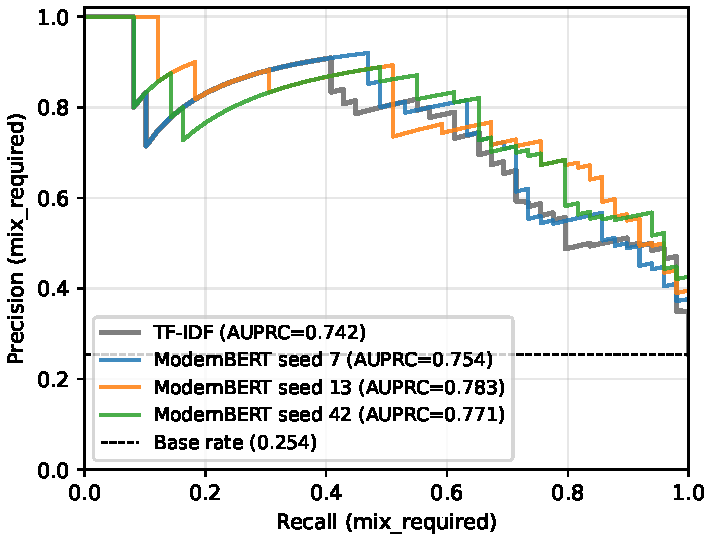
\includegraphics[width=0.85\textwidth]{figures/thesis/pr_curve_test.pdf}
\caption{Precision--recall curves on the held-out test split for the \gls{tfidf} baseline and the three ModernBERT training seeds. The dashed horizontal line is the test-set base rate of \texttt{mix\_required}.}
\label{fig:prCurveTest}
\end{figure}

\begin{figure}[!ht]
\centering
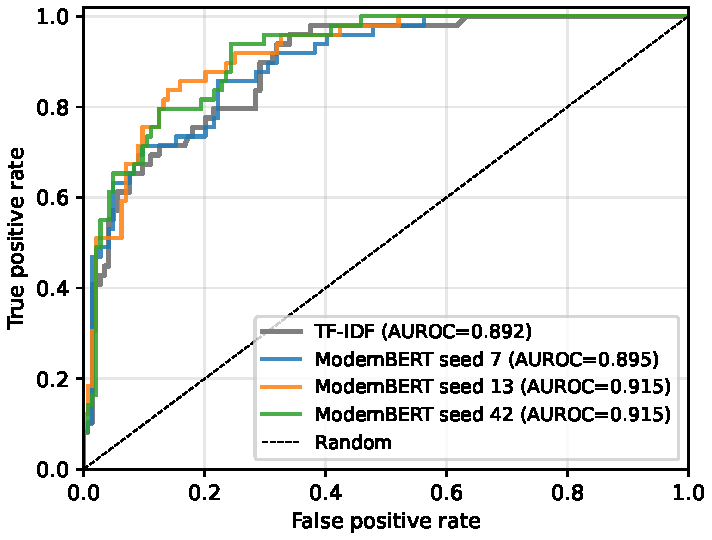
\includegraphics[width=0.85\textwidth]{figures/thesis/roc_curve_test.pdf}
\caption{Receiver-operating-characteristic curves on the held-out test split.}
\label{fig:rocCurveTest}
\end{figure}

Figure~\ref{fig:thresholdVsF1} shows how F1 on \texttt{mix\_required} varies with the decision threshold on the test split, with the validation-selected threshold of each model marked as a dot. The ModernBERT seeds select different thresholds. Seed $42$ selects $\tau^\star = 0.24$, seed $7$ selects $\tau^\star = 0.36$, and seed $13$ selects $\tau^\star = 0.42$. Their test F1 at the chosen threshold is nevertheless consistent (mean $0.699$, standard deviation $0.017$), suggesting the F1 plateau is broad and the routers degrade gracefully when the threshold is mistuned.

\begin{figure}[!ht]
\centering
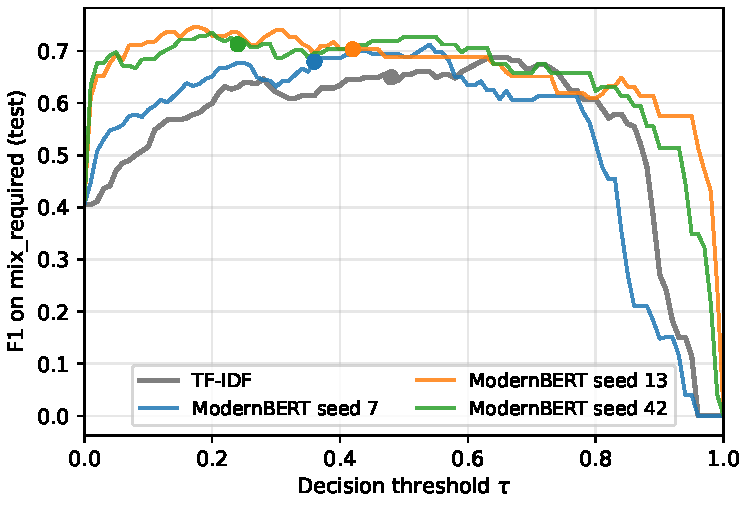
\includegraphics[width=0.85\textwidth]{figures/thesis/threshold_vs_f1_mix.pdf}
\caption{F1 on \texttt{mix\_required} as a function of the decision threshold on the held-out test split. Dots mark the validation-selected threshold for each model: TF-IDF $\tau^\star = 0.48$, ModernBERT seed $42$ $\tau^\star = 0.24$, seed $7$ $\tau^\star = 0.36$, seed $13$ $\tau^\star = 0.42$.}
\label{fig:thresholdVsF1}
\end{figure}

Figure~\ref{fig:thresholdVsTime} shows the mean routed time on test as the threshold sweeps from $0$ (every query routed to \emph{Mix}) to $1$ (every query routed to \emph{Naive}). The always-\emph{Naive} and always-\emph{Mix} levels are shown as horizontal dashed lines and act as a sanity check. At $\tau = 0$ every router collapses to always-\emph{Mix}, and at $\tau = 1$ every router collapses to always-\emph{Naive}, which is what the figure shows.

\begin{figure}[!ht]
\centering
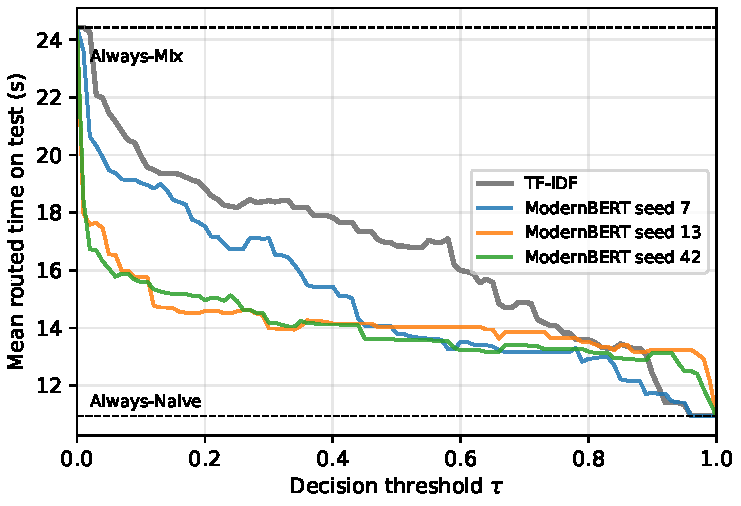
\includegraphics[width=0.85\textwidth]{figures/thesis/threshold_vs_routed_time.pdf}
\caption{Mean routed execution time on the held-out test split as the decision threshold sweeps. The two horizontal dashed lines are the always-\emph{Naive} and always-\emph{Mix} reference levels.}
\label{fig:thresholdVsTime}
\end{figure}

Figure~\ref{fig:costFrontier} combines the two preceding views into a cost--performance frontier. Each router traces a Pareto curve in (mean routed time, F1\textsubscript{mix}) space as $\tau$ sweeps. The static always-\emph{Naive} and always-\emph{Mix} policies appear as the two extreme operating points. The validation-selected operating points for the learned routers lie above the straight line connecting the two static endpoints. This is the operating range in which a router is useful, providing operating points that no static policy can reach by itself. The ModernBERT router lies slightly above and to the right of the \gls{tfidf} baseline, reaching higher F1\textsubscript{mix} at a slightly higher mean routed time.

\begin{figure}[!ht]
\centering
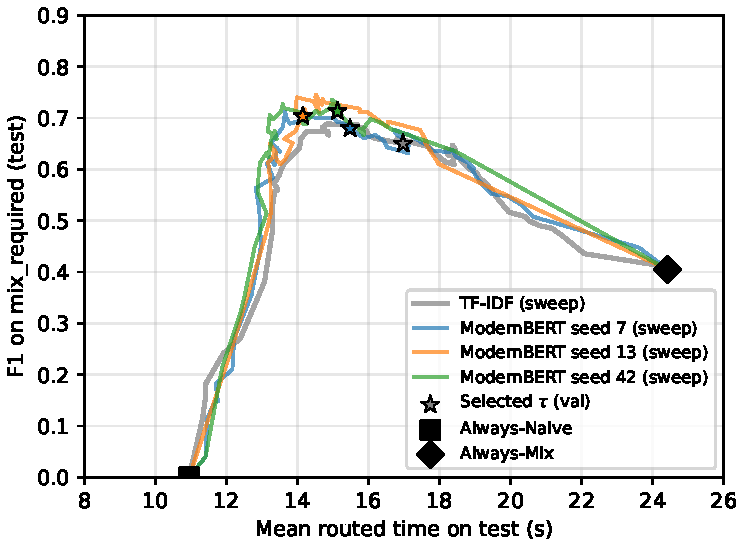
\includegraphics[width=0.85\textwidth]{figures/thesis/cost_performance_frontier.pdf}
\caption{Cost--performance frontier on the held-out test split. Each curve traces F1 on \texttt{mix\_required} versus mean routed execution time as the decision threshold sweeps. Stars mark the validation-selected operating point of each router. The black square (always-\emph{Naive}) and the black diamond (always-\emph{Mix}) are the two static baselines.}
\label{fig:costFrontier}
\end{figure}

Table~\ref{tab:perQuestionType} reports a per-question-type breakdown on the test split. The 2WikiMultihopQA question types have very different routing distributions. The \texttt{comparison} slice is almost always \texttt{naive\_enough}, with only $2$ of $90$ test rows requiring \emph{Mix}. The \texttt{bridge\_comparison} slice sits around one quarter. The \texttt{compositional} slice is the one in which the routing decision matters most, with $38$ of $65$ test rows requiring \emph{Mix}. The \texttt{inference} slice contributes only $5$ test rows, of which one is \texttt{mix\_required}, so its per-class metrics are reported for completeness but should be read as a description of these particular test rows rather than as a stable estimate. On the \texttt{compositional} slice ModernBERT improves \gls{auprc} over \gls{tfidf} (mean $0.839$ vs.\ $0.814$) and F1 on \texttt{mix\_required} (mean $0.799$ vs.\ $0.753$). On \texttt{bridge\_comparison} the picture is more mixed. \gls{tfidf} achieves a slightly higher \gls{auprc} and F1 here ($0.418$ and $0.316$) by routing more queries to \emph{Mix} on this slice, while ModernBERT is more conservative, with lower recall ($0.167$ vs.\ $0.375$) but higher precision ($0.345$ vs.\ $0.273$) and higher overall slice accuracy ($0.707$ vs.\ $0.606$).

\begin{table}[!ht]
\centering
\caption{Per-question-type breakdown on the test split. \texttt{P\textsubscript{mix}}, \texttt{R\textsubscript{mix}}, and \texttt{F1\textsubscript{mix}} denote precision, recall, and F1 on the \texttt{mix\_required} class. \Gls{auprc} values on the \texttt{comparison} and \texttt{inference} slices are computed on too few \texttt{mix\_required} positives to be informative and should be read as a description of these particular test rows rather than as a stable estimate. ModernBERT values are the mean over three seeds.}
\label{tab:perQuestionType}
\begin{tabular}{l|rrrrrrrr}
\textbf{Slice} & \textbf{n} & \textbf{n\textsubscript{mix}} & \textbf{Model} & \textbf{AUPRC} & \textbf{P\textsubscript{mix}} & \textbf{R\textsubscript{mix}} & \textbf{F1\textsubscript{mix}} & \textbf{Acc.} \\
\hline
comparison        &  90 &  2 & TF-IDF     & 0.277 & 0.000 & 0.000 & 0.000 & 0.978 \\
                  &     &    & ModernBERT & 0.237 & 0.000 & 0.000 & 0.000 & 0.978 \\
\hline
compositional     &  65 & 38 & TF-IDF     & 0.814 & 0.636 & 0.921 & 0.753 & 0.646 \\
                  &     &    & ModernBERT & 0.839 & 0.741 & 0.868 & 0.799 & 0.744 \\
\hline
bridge\_comparison&  33 &  8 & TF-IDF     & 0.418 & 0.273 & 0.375 & 0.316 & 0.606 \\
                  &     &    & ModernBERT & 0.363 & 0.345 & 0.167 & 0.211 & 0.707 \\
\hline
inference         &   5 &  1 & TF-IDF     & 0.333 & 0.000 & 0.000 & 0.000 & 0.400 \\
                  &     &    & ModernBERT & 0.833 & 0.000 & 0.000 & 0.000 & 0.733 \\
\end{tabular}
\end{table}

Figure~\ref{fig:perQt} visualizes the \gls{auprc} comparison on the two non-degenerate slices.

\begin{figure}[!ht]
\centering
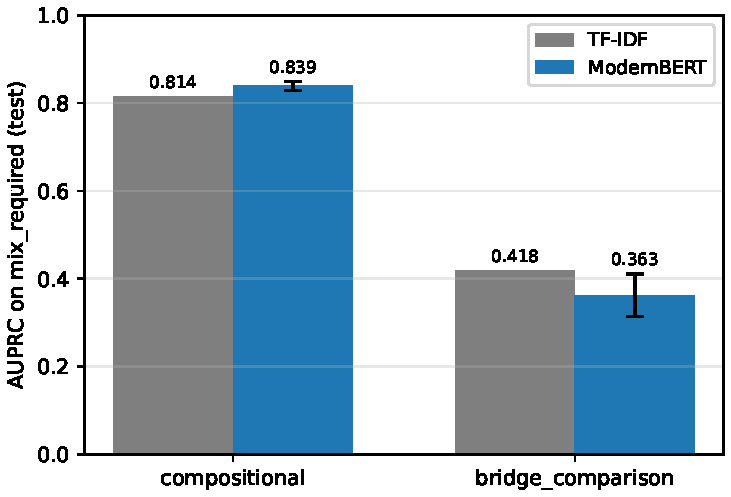
\includegraphics[width=0.85\textwidth]{figures/thesis/per_question_type_auprc.pdf}
\caption{\Gls{auprc} on the \texttt{mix\_required} class, broken down by 2WikiMultihopQA question type on the held-out test split. ModernBERT bars show the mean over three training seeds with error bars at one standard deviation. The \texttt{comparison} and \texttt{inference} slices have too few \texttt{mix\_required} test rows to give an informative \gls{auprc} and are omitted.}
\label{fig:perQt}
\end{figure}

\section{Discussion}
\label{sec:implDiscussion}

The headline result is that the retrieval-mode distinction between \emph{Naive} and \emph{Mix} is partly predictable from the query text alone. Both routers comfortably outperform the always-\emph{Naive} majority baseline on the minority class and reach operating points that are not on the straight line between the two static policies in Figure~\ref{fig:costFrontier}. The ModernBERT router is consistently better than the \gls{tfidf} baseline on \gls{auprc}, balanced accuracy, F1 on the minority class, and overall accuracy, with differences that are stable across three training seeds.

The most informative slice is \texttt{compositional}. This is where the class distribution is balanced and where graph-enhanced retrieval is most often needed. On this slice ModernBERT achieves a mean \gls{auprc} of $0.839$ against \gls{tfidf}'s $0.814$ and lifts F1 on \texttt{mix\_required} from $0.753$ to $0.799$, despite the small training set, which suggests that the encoder picks up on more than the lexical patterns a \gls{tfidf} classifier can exploit. The \texttt{bridge\_comparison} slice is harder for both routers. \gls{tfidf} reaches a slightly higher \gls{auprc} and F1 here ($0.418$ and $0.316$) by routing more queries to \emph{Mix} on this slice, while ModernBERT is more conservative on this slice and ends up with higher slice accuracy ($0.707$ vs.\ $0.606$) and higher precision but lower minority recall. Neither outcome is satisfactory, and improving routing on this slice is an obvious target for further work.

There are limitations to the headline result. The held-out test set has 193 queries, which is enough to compute meaningful bootstrap intervals but not enough to resolve small differences between the routers. \gls{tfidf}'s bootstrap \gls{auroc} interval ($[0.836, 0.936]$) contains the ModernBERT mean \gls{auroc} of $0.908$, so the \gls{auroc} comparison cannot be called significant on this test set. The \gls{auprc} and balanced-accuracy gaps are larger but still inside the bootstrap intervals, which is what should be expected on a $193$-row test set. The multi-seed standard deviation for ModernBERT is small ($0.015$ on \gls{auprc}, $0.012$ on balanced accuracy, $0.017$ on F1), so the gains are at least stable across seeds, but a larger benchmark would be needed before stronger claims can be made.

The cost picture is even more pronounced in LLM tokens than in execution time. The two static baselines bracket a mean routed range of $11.0$ to $24.4$ seconds per query in execution time and roughly $3{,}500$ to $17{,}900$ tokens per query in LLM usage. The learned routers select operating points around $15$ to $17$ seconds (a $30$--$39\,\%$ reduction in time relative to always-\emph{Mix}) and $7{,}100$ to $8{,}500$ tokens (a $52$--$60\,\%$ reduction in tokens relative to always-\emph{Mix}), at non-trivial \texttt{mix\_required} F1. The token saving is more dramatic than the time saving because \emph{Mix} adds one extra LLM call per query and a substantially larger assembled context \cite{lightrag2024,microsoft2024graphragcosts}, whereas time is partly absorbed by network latency that is independent of token volume. The routing decision itself contributes essentially zero LLM tokens, since neither router calls a generative model. It contributes only milliseconds of compute time, which is negligible next to retrieval cost on either dimension.

\cleardoublepage
\chapter{Conclusions and future work}
\label{ch:conclusionsAndFutureWork}

This chapter summarizes the conclusions from the experiments (Section~\ref{sec:conclusions}), discusses the main limitations and natural avenues for future work (Section~\ref{sec:limitationsFutureWork}), and reflects on the broader context of the project (Section~\ref{sec:reflections}).

\section{Conclusions}
\label{sec:conclusions}

This thesis studied whether the choice between LightRAG's cheap \emph{Naive} retrieval mode and its more expensive \emph{Mix} retrieval mode can be predicted from the query text alone, on the 2WikiMultihopQA benchmark, using a lightweight encoder-only classifier rather than a large language-model controller. Routing labels were derived by executing both retrieval modes on each benchmark question and using an \gls{llmjudge} \cite{zheng2023judge} to compare each mode's answer against the gold answer.

On the held-out test split, the ModernBERT router improves on a \gls{tfidf} logistic-regression baseline on \gls{auprc} ($0.769$ vs. $0.742$), balanced accuracy ($0.798$ vs. $0.784$), F1 on the minority \texttt{mix\_required} class ($0.699$ vs. $0.650$), and overall accuracy ($0.846$ vs. $0.788$), while remaining within the bootstrap interval on \gls{auroc}. The multi-seed standard deviation of the ModernBERT router is small on every aggregate classification metric ($\leq 0.017$ on \gls{auprc}, \gls{auroc}, balanced accuracy, F1, and accuracy), which makes the improvement stable rather than seed-specific. Both learned routers reach test-set operating points around $15$ to $17$ seconds of mean routed execution time, compared with $11.0$ seconds for always-\emph{Naive} and $24.4$ seconds for always-\emph{Mix}, and lie above the straight line connecting the two static endpoints in the cost--performance frontier. Measured in LLM tokens, the same routers route at roughly $7{,}100$ to $8{,}500$ mean tokens per query, compared with $3{,}458$ for always-\emph{Naive} and $17{,}857$ for always-\emph{Mix}, a routing saving of $52$--$60\,\%$ relative to the expensive baseline.

The per-question-type breakdown localizes most of the routing signal in the \texttt{compositional} slice, where graph-enhanced retrieval is most often needed ($58\,\%$ of the test slice) and where ModernBERT improves \gls{auprc} over \gls{tfidf} by roughly two and a half points. The \texttt{comparison} slice is essentially decidable as \emph{Naive} and both routers correctly avoid \emph{Mix} on it. The \texttt{bridge\_comparison} slice is the weakest part of the result and is the natural target for further work.

Returning to the research question, the distinction between vector-sufficient and graph-required queries is, in this setting, partly predictable from the query text alone. The gain over a classical baseline is small but stable, and the practical effect is non-trivial cost savings at a level of \texttt{mix\_required} recall that no static policy at comparable cost can reach.

\section{Limitations and future work}
\label{sec:limitationsFutureWork}

\subsection{Token-cost measurement scope}
\label{sec:limitTokenCost}

LLM token cost in this thesis is reported using per-mode mean token usage from an instrumented subset of $N=15$ queries spanning all four 2WikiMultihopQA question types, applied to the full test split to produce extrapolated routed-token figures. Token cost varies query to query depending on context size and retrieval breadth \cite{lightrag2024,microsoft2024graphragcosts}, so a small-N mean is an approximation rather than a per-query measurement. Per-query token logging across the full $1{,}286$-row routing dataset would give bootstrap confidence intervals for the routed-token saving directly comparable to those reported for execution time. Instrumenting LightRAG to log token usage on every retrieval call is a natural follow-up.

\subsection{Judge labels}
\label{sec:limitJudgeLabels}

Routing labels were produced by a single \gls{llmjudge} model with access to the gold answer. This is a reasonable but imperfect labeling protocol \cite{zheng2023judge}. The risk is that the judge systematically misclassifies particular kinds of correct answers, which would shift the routing labels in a way that the router learns to mimic. A natural follow-up is to label a sample of queries with a different judge model or with human annotators and measure inter-rater agreement on the routing label, both as a sanity check on the existing labels and as a more reliable evaluation subset.

\subsection{Generalizability}
\label{sec:limitGeneralizability}

The experiments use one Hybrid \gls{rag} framework (LightRAG), two of its retrieval modes (\emph{Naive} and \emph{Mix}), and one public benchmark (2WikiMultihopQA). The held-out test set has $193$ rows, which is enough to compute bootstrap intervals but not enough to resolve small differences between routers. The conclusions therefore apply most directly to the studied setting, and applying the same methodology to other Hybrid \gls{rag} frameworks (for example GraphRAG \cite{edge2024graphrag} or Hybrid retrieval modes in other systems) or to other multi-hop benchmarks (HotpotQA, MuSiQue \cite{yang2018hotpotqa,trivedi2022musique}) is a natural way to test how robust the routing signal is. Extending the routing labels to industrial corpora (for example Ericsson internal documentation) was considered but is blocked by the absence of per-query ground-truth answers in those corpora, which is what made the judge-labeling protocol possible on 2WikiMultihopQA in the first place.

\subsection{Routing beyond the query}
\label{sec:limitRouting}

The router used in this thesis is query-only by construction. A router that also has access to some lightweight signal from the corpus or from a cheap first retrieval pass could in principle make a better decision, at the cost of a slightly more expensive routing layer. A natural follow-up is to compare the query-only router against a hybrid scheme that first runs the cheap \emph{Naive} mode, inspects whether the retrieved chunks contain the entities referenced in the query, and then escalates to \emph{Mix} only when this signal looks weak, similar to how Adaptive-RAG conditions on cheap intermediate signals at the language-model level \cite{jeong2024adaptiverag}. This would still keep the routing layer cheap (one round of vector retrieval rather than an expensive graph traversal) but could materially improve the harder slices, in particular \texttt{bridge\_comparison}.

\subsection{Calibration and abstention}
\label{sec:limitCalibration}

The router currently outputs a single thresholded decision. Routing under cost constraints is a natural setting for selective prediction \cite{geifman2017selective} and calibrated probabilities \cite{guo2017calibration}, where the router could abstain on low-confidence queries (for example by escalating to a more expensive but more reliable controller, or by running both retrieval modes and combining the answers). The calibration of the ModernBERT router's softmax outputs was not investigated in this work and is a natural piece of follow-up.

\section{Reflections}
\label{sec:reflections}

This thesis is centered on making a Hybrid \gls{rag} system more resource-efficient. The most direct connection is to the \gls{UN} \gls{SDG} number 12 (responsible consumption and production). Graph-enhanced retrieval is significantly more compute-intensive than vector retrieval \cite{lightrag2024,microsoft2024graphragcosts}, and a router that avoids applying it to queries that do not need it directly reduces the energy and compute footprint of the system at inference time. There is also a softer connection to \gls{SDG} number 9 (industry, innovation, and infrastructure), in that adaptive routing is a building block for industrial \gls{rag} deployments such as the one motivating this work at Ericsson, where serving company-internal documentation at scale is a real operational concern.

The work has some ethical aspects worth flagging. The routing labels are produced by an \gls{llmjudge} that has access to the gold answer. This is a methodologically reasonable but imperfect protocol, and the thesis is explicit about not treating these labels as ground truth. Building a system that decides on a per-query basis which retrieval path to use could in principle interact with downstream notions of answer quality in ways that are hard to anticipate. If the router systematically routes some kind of question to the cheaper path, that kind of question could end up consistently worse-served, even when the average behavior of the system improves. The per-question-type breakdown in Section~\ref{sec:implResults} is one way to surface this kind of differential behavior, and any future work that scales this approach to user-facing settings should keep similar per-segment analyses in view.

\noindent\rule{\textwidth}{0.4mm}

\cleardoublepage
% Print the bibliography (and make it appear in the table of contents)
\renewcommand{\bibname}{References}


\iftoggle{biblatex}{
    %\typeout{Biblatex current language is \currentlang}
    \printbibliography[heading=bibintoc]
}{
    \phantomsection  % make it include a hyperref - see https://tex.stackexchange.com/a/98995
    \addcontentsline{toc}{chapter}{References}
    \bibliography{references}
}



\cleardoublepage
\appendix
\renewcommand{\chaptermark}[1]{\markboth{Appendix \thechapter\relax:\thinspace\relax#1}{}}
\chapter{Source code}
\label{sec:supportingMaterial}

The implementation code, the data-preparation pipeline, the training scripts, and the evaluation scripts used in this thesis are publicly available at \url{\thesisCodeUrl}.

\cleardoublepage

\begin{comment}
% If you actually want to have the full table of National Subject Categories (temporarily) include this appendix
\subfile{README_notes/National_Subject_Categories}
\cleardoublepage
\end{comment}

\begin{comment}
% Information for examiners
\ifxeorlua
\cleardoublepage
\input{README_notes/README_examiner_notes}
\fi
\end{comment}

\begin{comment}
% Information for administrators
\ifxeorlua
\cleardoublepage
\input{README_notes/README_for_administrators.tex}
\fi
\end{comment}

\begin{comment}
% Information for Course Coordinators
\ifxeorlua
\cleardoublepage
\input{README_notes/README_for_course_coordinators}
\fi
\end{comment}

%% The following label is necessary for computing the last page number of the body of the report to include in the "For DIVA" information
\label{pg:lastPageofMainmatter}

\cleardoublepage
\clearpage\thispagestyle{empty}\mbox{} % empty page with backcover on the other side
\kthbackcover

\end{document}
